\documentclass[10pt, oneside]{article} 
\usepackage{amsmath, amsthm, amssymb, calrsfs, wasysym, verbatim, bbm, color, graphics, graphicx, geometry, tocloft, subcaption, blindtext, hyperref, array}

\geometry{tmargin=.75in, bmargin=.75in, lmargin=.75in, rmargin = .75in}  

\newcommand{\R}{\mathbb{R}}
\newcommand{\C}{\mathbb{C}}
\newcommand{\Z}{\mathbb{Z}}
\newcommand{\N}{\mathbb{N}}
\newcommand{\Q}{\mathbb{Q}}
\newcommand{\Cdot}{\boldsymbol{\cdot}}

% comment command
\newcommand{\Comment}[1]{\noindent \textcolor{blue}{\textit{#1}} \par}

\newtheorem{thm}{Theorem}
\newtheorem{defn}{Definition}
\newtheorem{conv}{Convention}
\newtheorem{rem}{Remark}
\newtheorem{lem}{Lemma}
\newtheorem{cor}{Corollary}

\setlength{\parindent}{0pt}


\title{Security \& Cryptography Class Notes}
\author{Anna Visman}
\date{Academic Year 2024-2025}

\begin{document}

\maketitle
\tableofcontents

\vspace{.25in}

\newpage 
\section{Lecture 1}

\subsection{Security Overview}

A computer system is said to be secure if it satisfies the following properties:
\begin{itemize}
\item {\bf Confidentiality}: Unauthorized entities cannot access the system or its data
\item {\bf Integrity}: When you receive data, it is the right one
\item {\bf Availability}: The system or data is there when you need it
\end{itemize}

\begin{rem}
The mere presence of these properties does not necessarily mean that the system is fully secure in practice.
\end{rem}

A secure system is reliable:

\begin{itemize}
    \item Keep your personal data confidential 
    \item Allow only authorised access or modifications to resources
    \item Ensure that any produced results are correct
    \item Give you correct and meaningful results whenever you want them
\end{itemize}


Terminology:

\begin{itemize}
    \item {\bf{Assets}}: Things we want to protect (hardware, software, data)
    \item {\bf{Vulnerabilities}}: Weaknesses in a system that may be exploited in order to cause loss and harm
    \item {\bf{Threats}}: A loss or harm that might befall a system (interception, interruption, modification, fabrication)
    \item {\bf{Attack}}: An action which exploits a vulnerability to execute a threat 
    \item {\bf{Control/Defence}}: Removing/reducing a vulnerability. You control a vulnerability to prevent an attack and defend against a threat
\end{itemize}

Methods of Defence:

\begin{itemize}
    \item Prevent it
    \item Deter it: make the attack harder or more expensive
    \item Deflect it: make yourself less attractive to attacker
    \item Detect it: notice that the attack is occurring
    \item Recover from it: mitigate the effects of the attack
\end{itemize}

Principle of Easiest Penetration: A system is only as secure as its weakest link. An attacker will go after whatever part of the system is easiest for them, not most convenient for you. In order to build secure systems, we need to learn how to think like an attacker!

\subsection{Defense Overview}
Software controls:
\begin{itemize}
    \item Passwords and other forms of access control
    \item Operating systems separate users' actions from each other
    \item Virus scanner watch for malware
    \item Development controls enforce quality measures on the original source code 
    \item Personal firewalls that run on your desktop
\end{itemize}

Hardware controls:
\begin{itemize}
    \item Not usually protection of the hardware itself, but rather using separate hardware to protect the system as a whole 
    \item Fingerprint readers
    \item Smart tokens
    \item Firewalls
    \item Intrusion detection systems
\end{itemize}

Physical Systems:
\begin{itemize}
    \item Protection of the hardwell itself, as well as physical access to the console, storage media, etc.
    \item Locks
    \item Guards
    \item Off-site backups
\end{itemize}

Policies and Procedures:
\begin{itemize}
    \item Non-technical means can be used to protect against some classes of attack (e.g. VPNs for accessing interal company network)
    \item Rules about choosing Passwords
    \item Training in best security practices
\end{itemize}

\subsection{Cryptography Overview}
Objectives of Cryptography:
\begin{itemize}
    \item Protecting data privacy
    \item Authenticaion (message, data origin, entity)
    \item Non-repudiation: preventing the sender from later denying that they sent the message
\end{itemize}

\newpage

\begin{defn}
Kerkhoff's Principle: The adversary knows all details about a crypto system except the secret key.
\end{defn}

\begin{defn}
Cipher: A method or algorithm used to transform readable data (called plaintext) into an unreadable format (called ciphertext) to protect its confidentiality.
\end{defn}

Encryption is the process of converting plaintext into ciphertext. Decryption is the reverse process. Encryption uses the key k, decryption uses the key k'. If k = k', the system is symmetric. If k $\neq$ k', the system is asymmetric. Decryption(Encryption(m)) = m.
\begin{figure}[h!]
    \centering
    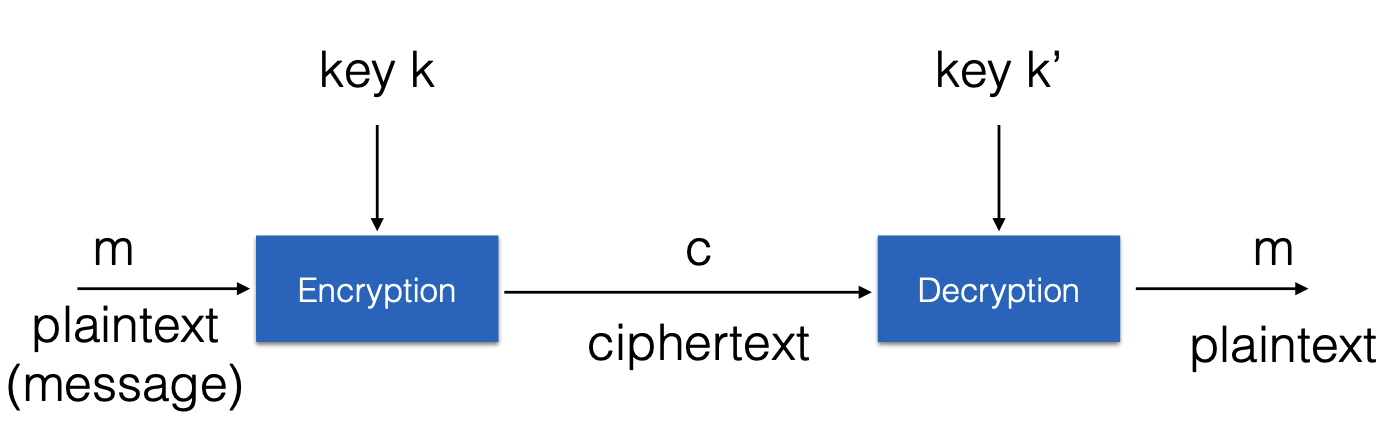
\includegraphics[scale=0.5]{img/w1encryption.png}
    \caption{Encryption}
\end{figure}

\begin{table}[h!]
    \centering
    \begin{tabular}{|l|l|l|}
    \hline
    \textbf{Feature}        & \textbf{Private Key Encryption}        & \textbf{Public Key Encryption}         \\ \hline
    \textbf{Keys}           & Same key for encryption \& decryption  & Two keys: public and private           \\ \hline
    \textbf{Speed}          & Faster                                 & Slower                                 \\ \hline
    \textbf{Key sharing}    & Must be kept secret                    & Only the private key is secret         \\ \hline
    \textbf{Use cases}      & Encrypting large data, e.g., files     & Secure key exchange, digital signatures \\ \hline
    \end{tabular}
    \caption{Summary of Differences Between Private and Public Key Encryption}
    \label{tab:encryption_comparison}
    \end{table}
    
\subsection{Topics Covered in Course}
\begin{itemize}
\item Classical systems: simple ciphers, substitution, permutation, transposition, Caesar, Vigenere
\item Information Theoretic Security
\item Defining security: pseudorandomness, one-way functions, trapdoor functions
\item Notions of security: perfect secrecy, semantic security, IND security
\item Attacks on encryption schemes: objective, levels of computing power, amount of information available
\item Types attacks: ciphertext-only, known plaintext, chosen plaintext, chosen ciphertext, adaptive
\item Different types of adversaries: unbounded/polynomial computing power
\item Security: unconditionally secure, computationally secure
\item and more... see slides
\end{itemize}


\newpage

\section{Lecture 2}

\newcommand{\floor}[1]{\left\lfloor #1 \right\rfloor}

\subsection{Number Theory}

\subsubsection{Modular Arithmetic}
\begin{defn}
A positive integer \( N \) is called the \emph{modulus}. Two integers \( a \) and \( b \) are said to be congruent modulo \( N \), written \( a \equiv b \pmod{N} \), if \( N \) divides \( b - a \).
\end{defn}    

Examples:
\[
18 \equiv 4 \pmod{7}, \quad -18 \equiv 3 \pmod{7}.
\]

The set of integers modulo \( N \) is denoted by \( \mathbb{Z}/N\mathbb{Z} \) or \( \mathbb{Z}_N \):
\[
\mathbb{Z}/N\mathbb{Z} = \{ 0, 1, \dots, N-1 \}, \quad \#(\mathbb{Z}/N\mathbb{Z}) = N.
\]

Properties of Modular Arithmetic:
\begin{enumerate}
    \item Addition is closed: \(\forall a, b \in \mathbb{Z}/N\mathbb{Z} : a + b \in \mathbb{Z}/N\mathbb{Z}\).
    \item Addition is associative: \(\forall a, b, c \in \mathbb{Z}/N\mathbb{Z} : (a + b) + c = a + (b + c)\).
    \item \(0\) is an additive identity: \(\forall a \in \mathbb{Z}/N\mathbb{Z} : a + 0 = 0 + a = a\).
    \item The additive inverse always exists: \(\forall a \in \mathbb{Z}/N\mathbb{Z} : a + (N - a) = (N - a) + a = 0\).
    \item Addition is commutative: \(\forall a, b \in \mathbb{Z}/N\mathbb{Z} : a + b = b + a\).
    \item Multiplication is closed: \(\forall a, b \in \mathbb{Z}/N\mathbb{Z} : a \cdot b \in \mathbb{Z}/N\mathbb{Z}\).
    \item Multiplication is associative: \(\forall a, b, c \in \mathbb{Z}/N\mathbb{Z} : (a \cdot b) \cdot c = a \cdot (b \cdot c)\).
    \item \(1\) is a multiplicative identity: \(\forall a \in \mathbb{Z}/N\mathbb{Z} : a \cdot 1 = 1 \cdot a = a\).
    \item Multiplication and addition satisfy the distributive law: \(\forall a, b, c \in \mathbb{Z}/N\mathbb{Z} : (a + b) \cdot c = a \cdot c + b \cdot c\).
    \item Multiplication is commutative: \(\forall a, b \in \mathbb{Z}/N\mathbb{Z} : a \cdot b = b \cdot a\).
\end{enumerate}

\subsubsection{Modular Exponentiation}
Modular exponentiation is a technique used to efficiently compute expressions of the form \( a^b \mod m \), especially for large \( b \). The key idea is to repeatedly square the base \( a \), reduce modulo \( m \) at each step, and combine results as needed. \\

\textbf{Example: Compute \( 3^4 \mod 11 \)}

\begin{enumerate}
    \item Write the problem:
    \[
    3^4 \mod 11
    \]
 
 \item Break it into smaller steps using properties of modular arithmetic:
 \begin{enumerate}
    \item First, compute \( 3^2 \mod 11 \):
    \[
    3^2 = 9 \quad \Rightarrow \quad 9 \mod 11 = 9
    \]
    \item Then, square the result to get \( 3^4 \mod 11 \):
    \[
    3^4 = (3^2)^2 = 9^2 = 81 \quad \Rightarrow \quad 81 \mod 11 = 4
    \]
 \end{enumerate}
 
 \item Final result:
    \[
    3^4 \mod 11 = 4
    \]
 
\end{enumerate}
 
\textbf{General Algorithm: Exponentiation by Squaring}
\begin{enumerate}
    \item If \( b \) is even:
    \[
    a^b \mod m = \left( a^{b/2} \mod m \right)^2 \mod m
    \]
    \item If \( b \) is odd:
    \[
    a^b \mod m = \left( a \cdot a^{b-1} \mod m \right) \mod m
    \]
\end{enumerate}

You can also simplify the problem by reducing the base modulo:
\begin{defn}
    For any a, b, n, if $a \equiv b \pmod{n}$, then $a^k \equiv b^k \pmod{n}$ for any positive integer k.
\end{defn}
See an example of this in practice session 1 exercise 1e. 

\subsubsection{Groups and Rings}
\begin{defn}
    A \emph{group} is a set with an operation that is:
    \begin{itemize}
        \item Closed,
        \item Has an identity element,
        \item Associative, and
        \item Each element has an inverse.
    \end{itemize}
    \end{defn}
    
    \begin{defn}
    A group is \emph{abelian} if it is also commutative.
    \end{defn}
    
    Examples:
    \begin{itemize}
        \item The integers under addition (\( \mathbb{Z}, + \)), where the identity is \( 0 \) and the inverse of \( x \) is \( -x \).
        \item The nonzero rationals under multiplication (\( \mathbb{Q}^*, \cdot \)), where the identity is \( 1 \) and the inverse of \( x \) is \( 1/x \).
    \end{itemize}


Group types:
\begin{itemize}
    \item Multiplicative group: operation is multiplication.
    \item Additive group: operation is addition.
    \item Cyclic abelian group: generated by a single element.
\end{itemize}

\begin{defn}
An abelian group G is called \emph{cyclic} if there exists an element in the group, called the \emph{generator}, from which every other element in G can be obtained either by repeated application of the group operation to the generator, or by the use of the inverse operation.
\begin{itemize}
    \item If the group operation is multiplication ($(G, \cdot)$), a generator $g$ produces all elements by repeated multiplication or division: $h = g^x$, where $h$ is an arbitrary element in the group.  
    \item In modular arithmetic, $g$ is a generator if $g^x \mod m $ produces all nonzero elements of the group as $x$ varies.
\end{itemize}
\end{defn}

\textbf{Example:} The group \( \mathbb{Z}_7^* \) (the multiplicative group of integers modulo \( 7 \)) consists of the nonzero integers modulo \( 7 \) under multiplication. The elements of the group are:
\[
\mathbb{Z}_7^* = \{ 1, 2, 3, 4, 5, 6 \}.
\]

An element \( g \in \mathbb{Z}_7^* \) is a generator if the powers \( g^x \mod 7 \) (for \( x = 1, 2, 3, \dots, 6 \)) produce \textbf{all elements} of \( \mathbb{Z}_7^* \) exactly once. Let's test whether \( 3 \) is a generator:

\begin{enumerate}
    \item Compute the powers of \( 3 \) modulo \( 7 \):
    \[
    3^1 \mod 7 = 3,
    \]
    \[
    3^2 \mod 7 = 9 \mod 7 = 2,
    \]
    \[
    3^3 \mod 7 = 27 \mod 7 = 6,
    \]
    \[
    3^4 \mod 7 = 81 \mod 7 = 4,
    \]
    \[
    3^5 \mod 7 = 243 \mod 7 = 5,
    \]
    \[
    3^6 \mod 7 = 729 \mod 7 = 1.
    \]

    \item The results are:
    \[
    \{ 3, 2, 6, 4, 5, 1 \}.
    \]
\end{enumerate}

Since this list contains all elements of \( \mathbb{Z}_7^* \), \( 3 \) is a generator of \( \mathbb{Z}_7^* \). Other generators of \( \mathbb{Z}_7^* \) include \( 5 \). You can verify this by computing \( 5^x \mod 7 \) for \( x = 1, 2, \dots, 6 \).

\begin{defn}
    A \emph{ring} is a set with two operations (\(+\), \(\cdot\)) satisfying:
    \begin{itemize}
        \item The set is an abelian group under addition.
        \item Multiplication is associative and closed.
        \item Distributive laws hold.
    \end{itemize}
    \end{defn}

If multiplication is commutative, the ring is called \emph{commutative}. Examples:
\begin{itemize}
        \item Integers, real numbers, and complex numbers form infinite rings.
        \item \( \mathbb{Z}/N\mathbb{Z} \) forms a finite ring.
\end{itemize}
    
\subsubsection{Primes and Divisibility}
\begin{defn}
    An integer \( a \) divides another integer \( b \), denoted \( a \mid b \), if \( b = k \cdot a \) for some integer \( k \).
    \end{defn}
    
\begin{defn}
    A number \( p \) is \emph{prime} if its only divisors are \( 1 \) and \( p \).
    \end{defn}
    
Examples of primes: \( 2, 3, 5, 7, 11, \dots \).

\begin{defn}
Greatest Common Divisor: \( c = \gcd(a,b) \) if and only if \( c \) is the largest number that divides
both \( a \) and \( b \).
\end{defn}

\begin{thm}
Every positive integer can be written as a product of primes in a unique way.
\end{thm}

\begin{defn}
Two integers a and b are coprime, relatively prime or mutually prime if the only positive integer that is a divisor of both of them is 1.
\end{defn}

\begin{defn}
Euler's Totient Function: \( \phi(p) \) is the number of integers less than \( p \) that are relatively prime to \( p \).
\begin{itemize}
    \item If N is a prime then \( \phi(N) = N - 1 \).
    \item If p and q are both prime and \( p \neq q \), then \( \phi(pq) = (p-1)(q-1)\)
\end{itemize}

\[ \phi(N) = N \left(1 - \frac{1}{p_1}\right) \left(1 - \frac{1}{p_2}\right) \ldots \left(1 - \frac{1}{p_k}\right) = n \prod_{p | n} (1 - \frac{1}{p})\]

where \( p_1, p_2, \ldots, p_k \) are the prime factors of \( N \).
\end{defn}

Euler's Totient function counts the number of positive up to a given integer N that are relatively prime to N. \\

\subsubsection{Linear Congruences}
\textbf{Finding the solution to the linear congruence equation:} \[ a \cdot x \equiv b \pmod{N}\]

We want to know how many solutions exist for x modulo N given the coefficients a, b, and the modulus N.

\begin{enumerate}
    \item Compute the greatest common divisor (\(\gcd\)) of \(a\) and \(N\), denoted as \(\gcd(a, N) = g\).
    \item The following cases determine the number of solutions:
    \begin{enumerate}
        \item \textbf{If \(g = 1\):}
        \begin{itemize}
            \item When \(a\) and \(N\) are coprime (\(\gcd(a, N) = 1\)), the equation has \textbf{exactly one solution} modulo \(N\). This is because \(a\) has a multiplicative inverse modulo \(N\).
        \end{itemize}
        
        \item \textbf{If \(g > 1\) and \(g \mid b\):}
        \begin{itemize}
            \item If \(\gcd(a, N) = g > 1\) and \(g\) divides \(b\), then there are \textbf{exactly \(g\) solutions} modulo \(N\).
            \item These solutions can be determined by reducing the equation to a simpler congruence modulo \(N/g\).
        \end{itemize}
        
        \item \textbf{If \(g > 1\) and \(g \nmid b\):}
        \begin{itemize}
            \item If \(g\) does not divide \(b\), then the equation has \textbf{no solution}. This is because \(b\) is not in the span of \(a\) modulo \(N\).
        \end{itemize}
    \end{enumerate}
\end{enumerate}

\begin{defn}
    Multiplicative Inverse Modulo N: A number that, when multiplied by a given number a, gives a result of 1 modulo N. In other words, the multiplicative inverse of \(a \) modulo N is a number \(x \) such that:
    \[ a \cdot x \equiv 1 \pmod{N} \]

    \begin{itemize}
        \item The multiplicative inverse of \(a\) modulo \(N\) is denoted as \(a^{-1}\).
        \item A multiplicative inverse of \(a\) modulo \(N\) exists only if \(a\) and \(N\) are coprime, i.e., \(\gcd(a, N) = 1\).

        \item If \(a\) and \(N\) are not coprime, it’s impossible to find \(x\) such that
        \(
        a \cdot x \equiv 1 \pmod{N}.
        \)
        \item When N is a prime p, then for all non-zero values of \( a \in \mathbb{Z}/p\mathbb{Z} \) we always obtain a unique solution to the equation \( a \cdot x \equiv 1 \pmod{p} \).
        
    \end{itemize}
\end{defn}

Inverse in this case means that the two numbers multiply to 1 modulo N. Think about regular numbers: the inverse of 2 is \( \frac{1}{2}\) under multiplication, because \( 2* \frac{1}{2} = 1\). 

\subsubsection{Fields}
\begin{defn}
A field is a set G with two operations \((G, \cdot, +) \). It satisfies the following properties:
\begin{itemize}
    \item \((G, +)\) is an abelian group with identity element 0 (G is a commutative group under addition).
    \item \((G \backslash \{0\}, \cdot)\) is an abelian group (\(G \backslash \{0\}\) is a commutative group under multiplicatio).
    \item Multiplication distributes over addition, i.e., \( (G, \cdot, +) \) satisfies the distributive law.
    \end{itemize}
\end{defn}

A field is like the "ideal playground" for numbers: You can add, subtract, multiply, and divide (except by 0). Both addition and multiplication behave nicely (associative, commutative, etc.). Examples of fields include familiar systems like real numbers and rational numbers.
The key difference between rings and fields is that in a ring, division is not always possible. In a field, division (except by 0) is always possible, because every nonzero element has a multiplicative inverse.

\[ \mathbb{Z}/N\mathbb{Z} \] is a field if and only if N is prime (because then every nonzero element has a multiplicative inverse). Else, it is a ring. 

Think of \(\mathbb{Z}/N\mathbb{Z}\) as a "clock" with \(N\) hours. Once you pass \(N-1\), you wrap around back to \(0\). Arithmetic in \(\mathbb{Z}/N\mathbb{Z}\) always "cycles" within the set \(\{0, 1, \dots, N-1\}\). \\

\( (\mathbb{Z}/N\mathbb{Z})^* \) is the set of all elements that are invertible (the set of elements that are coprime to N). 

\[ (\mathbb{Z}/N\mathbb{Z})^* = \{ x \in \mathbb{Z}/N\mathbb{Z} : \gcd{(x, N)} = 1 \}\] 

The size of \( (\mathbb{Z}/N\mathbb{Z})^* \) is given by Euler's Totient function: \( \phi(N) \). If N is a prime p, then \( (\mathbb{Z}/N\mathbb{Z})^*  = \{1, ..., p-1 \}\).

\subsubsection{Lagrange's Theorem}
Lagrange's Theorem states that if \((G, \cdot)\) is a finite group with order (size) \(n = \#G\), then for any element \(a \in G\), the order of \(a\) (the smallest positive integer \(k\) such that \(a^k = 1\)) divides \(n\). In particular, it follows that:
\[
a^n = 1 \quad \text{for all } a \in G.
\]

\textbf{Application in Modular Arithmetic:}  
In the context of modular arithmetic, consider the group of units \(\mathbb{Z}/N\mathbb{Z}^*\) (the set of integers modulo \(N\) that are coprime to \(N\), with multiplication as the group operation). If \(x \in \mathbb{Z}/N\mathbb{Z}^*\), then the group has size \(\phi(N)\), where \(\phi(N)\) is Euler's totient function (the count of integers less than \(N\) that are coprime to \(N\)). Therefore:
\[
x^{\phi(N)} \equiv 1 \pmod{N}.
\]

\subsubsection{Fermat's Little Theorem}
Fermat's Little Theorem states that if \(p\) is a prime number and \(a\) is any integer, then:
\[
a^p \equiv a \pmod{p}.
\]

If \(a\) is not divisible by \(p\), then this can be rewritten as:
\[
a^{p-1} \equiv 1 \pmod{p}.
\]

\textbf{Explanation:}  
This theorem tells us that raising \(a\) to the power of \(p-1\) gives a remainder of \(1\) when divided by \(p\), provided \(a\) and \(p\) are coprime. Fermat's Little Theorem is useful for simplifying modular exponentiation and serves as a foundation for more advanced results like Euler's theorem.

\subsection{Basic Algorithms}

\subsubsection{Euclid's GCD Algorithm}

The \textbf{Greatest Common Divisor} (GCD) of two integers \(a\) and \(b\) is the largest integer \(d\) such that \(d\) divides both \(a\) and \(b\). \\

\textbf{Key Idea:} If we could factorize \(a\) and \(b\), we could easily determine their GCD. For example, consider:
\[
a = 2^4 \cdot 157 \cdot 4513^3, \quad b = 2^2 \cdot 157 \cdot 2269^3 \cdot 4513.
\]
Here, the GCD is given by:
\[
\text{gcd}(a, b) = 2^2 \cdot 157 \cdot 4513 = 2{,}834{,}164.
\]
However, computing prime factorizations is often impractical for large numbers. Instead, we use Euclid's Algorithm. \\

The Euclidean Algorithm is based on the principle:
\[
\text{gcd}(a, b) = \text{gcd}(a \mod b, b).
\]
The algorithm starts with two numbers \(a,b\), where \(a > b\). The remainder \(r = a \mod b\) is computed. Then, \(a\) is repeatedly replaced with \(b\) (the smaller number), and \(b\) with \(r\) (the remainder). This process continues until the remainder is \(0\). The last non-zero remainder (b) is the GCD of \(a\) and \(b\).

\textbf{Steps:}
\begin{enumerate}
    \item Let \(r_0 = a\) and \(r_1 = b\).
    \item Compute remainders \(r_2, r_3, \dots\) using:
    \[
    r_{i+2} = r_i \mod r_{i+1}, \quad \text{where } r_{i+2} < r_{i+1}.
    \]
    \item Stop when \(r_{m+1} = 0\). The GCD is \(r_m\).
\end{enumerate}

\textbf{Example:}
Compute \(\text{gcd}(21, 12)\):
\[
\begin{aligned}
\text{gcd}(21, 12) &= \text{gcd}(21 \mod 12, 12) = \text{gcd}(9, 12), \\
\text{gcd}(9, 12) &= \text{gcd}(12 \mod 9, 9) = \text{gcd}(3, 9), \\
\text{gcd}(3, 9) &= \text{gcd}(9 \mod 3, 3) = \text{gcd}(0, 3).
\end{aligned}
\]
Thus, \(\text{gcd}(21, 12) = 3\).

\subsubsection{The Extended Euclidean Algorithm}
In addition to computing the GCD, the Extended Euclidean Algorithm finds integers \(x\) and \(y\) such that:
\[
\text{gcd}(a, b) = ax + by = r.
\]
This is useful in many applications, such as finding modular inverses. For \(
\text{gcd}(a, b) = d
\) where \(d = 1 \), we can compute \(ax + yN = 1 \). Here \textbf{x} is the multiplicative inverse of \(a\) in modulo N. So, if \(\text{gcd}(a, N) = 1\), then \(a^{-1} \mod N = x \mod N\). \\

\textbf{Algorithm:}
\begin{enumerate}
    \item Start with \(r_0 = a\), \(r_1 = b\), \(s_0 = 1\), \(s_1 = 0\), \(t_0 = 0\), \(t_1 = 1\).
    \item For each step, compute:
    \[
    q_i = \left\lfloor \frac{r_{i-1}}{r_i} \right\rfloor, \quad r_{i+1} = r_{i-1} - q_i r_i,
    \]
    \[
    s_{i+1} = s_{i-1} - q_i s_i, \quad t_{i+1} = t_{i-1} - q_i t_i.
    \]
    \item Stop when \(r_{i+1} = 0\). Then, \(\text{gcd}(a, b) = r_i\), and \(x = s_i\), \(y = t_i\).
    
\end{enumerate}

\textbf{Example:}
Compute \(\text{gcd}(36, 24)\) and coefficients \(x, y\):
\[
\begin{aligned}
&\text{Step 1: } q = \left\lfloor \frac{36}{24} \right\rfloor = 1, \quad r = 36 - 1 \cdot 24 = 12, \\
&\text{Update: } x = 0 - 1 \cdot 1 = -1, \quad y = 1 - 1 \cdot 0 = 1, \\
&\text{Step 2: } q = \left\lfloor \frac{24}{12} \right\rfloor = 2, \quad r = 24 - 2 \cdot 12 = 0, \\
&\text{Update: } x = 1 - 2 \cdot (-1) = 3, \quad y = 0 - 2 \cdot 1 = -2.
\end{aligned}
\]
Thus, \(\text{gcd}(36, 24) = 12\), with \(x = -1\), \(y = 1\).

\subsubsection{The Chinese Remainder Theorem}
Let \(m_1, ..., m_r \) be pairwise relatively prime (i.e., \(\gcd(m_i, m_j) = 1\) for all \(i \neq j\)). Let \(x = a_i \mod m_i \) for all i. The CRT guarantees a unique solution given by:

\[ x = \sum^r_{i=1} a_iM_iy_i \mod M\] 

where

\[ M_i = M \slash \ m_i\]

and 

\[ y_i = M^{-1}_i \mod m_i \] 

$y_i$ is the modular inverse of $M_i$ modulo  $m_i$ (this can be computed using the Extended Euclidean Algorithm). The theorem is a way to solve a system of simultaneous modular congruences, finding a unique solution for a number that satisfies multiple modular equations, provided that the moduli are coprime/relatively prime. 

\[ x \equiv a_1 \mod m_1 \] 
\[ x \equiv a_2 \mod m_2 \]
\[...\]
\[ x \equiv a_k \mod m_k \]

In that case, there exists a \textbf{unique solution} \(x\) modulo \(M\), where \(M\) is the product of all the moduli:

\[
M = m_1 \cdot m_2 \cdot \ldots \cdot m_k.
\]

\textbf{Example}:
\[x \equiv 5 \mod 7 \]
\[x \equiv 3 \mod 11 \]
\[x \equiv 10 \mod 13 \]

Then $ M = 7 \cdot 11 \cdot 13 = 1001$. $M_1 = 1001 \slash 7 = 143$, $M_2 = 1001 \slash 11 = 91$, $M_3 = 1001 \slash 13 = 77$. $y_1 = 5, y_2 = 4, y_3 = 12$.
\[ x = \sum^r_{i=1} a_iM_iy_i \mod M = 5 \cdot 143 \cdot 5 + 3 \cdot 91 \cdot 4 + 10 \cdot 77 \cdot 12 \mod 1001 \] 
\[= 3575 + 1092 + 9240 \mod 1001 = 13907 \mod 1001 = 894\]

\Comment{add here why we need the CRT}

\subsubsection{Computing Legendre and Jacobi Symbols}

\begin{defn}
    Let \( n \) be a positive integer. An integer \( a \) is called a \textbf{quadratic residue modulo \( n \)} if there exists an integer \( x \) such that:
    \[
    x^2 \equiv a \pmod{n}.
    \]
    In other words, \( a \) is a quadratic residue modulo \( n \) if \( a \) is congruent to the square of some integer \( x \) modulo \( n \).
    
    If no such \( x \) exists, then \( a \) is called a \textbf{quadratic non-residue modulo \( n \)}.    
\end{defn}

\textbf{Example:} For \( n = 7 \), the integers modulo \( 7 \) are \( \{ 0, 1, 2, 3, 4, 5, 6 \} \). Computing the squares of each integer modulo \( 7 \):
\[
\begin{aligned}
    0^2 &\equiv 0 \pmod{7}, \\
    1^2 &\equiv 1 \pmod{7}, \\
    2^2 &\equiv 4 \pmod{7}, \\
    3^2 &\equiv 2 \pmod{7}, \\
    4^2 &\equiv 2 \pmod{7}, \\
    5^2 &\equiv 4 \pmod{7}, \\
    6^2 &\equiv 1 \pmod{7}.
\end{aligned}
\]

The quadratic residues modulo \( 7 \) are:
\[
\{ 0, 1, 2, 4 \}.
\]

The quadratic non-residues modulo \( 7 \) are:
\[
\{ 3, 5, 6 \}.
\]
 
Symmetry of squares: squaring numbers modulo $n$ often produces repeated results due to symmetry in the group of residues. This means that different numbers can have the same square when considered modulo $n$. For each $x$, its symmetric counterpart $n-x$ produces the same square modulo $n$. The total number of unique quadratic residues is approximately half of $n$ (or $\floor{n\slash2} + 1$ if 0 is included).

\begin{defn}
    Legendre Symbol: Let \( p \) be a prime number, and let \( a \) be an integer. The \textbf{Legendre symbol} \( \left( \frac{a}{p} \right) \) is defined as follows:

    \[
    \left( \frac{a}{p} \right) =
    \begin{cases}
    1 & \text{if } a \text{ is a quadratic residue modulo } p \text{ and } a \not\equiv 0 \pmod{p}, \\
    -1 & \text{if } a \text{ is a quadratic non-residue modulo } p, \\
    0 & \text{if } p \mid a \text{ (i.e., if } a \equiv 0 \pmod{p}).
    \end{cases}
    \]
\end{defn}

\begin{itemize}
    \item \( \left( \frac{a}{p} \right) = 1 \) means there exists an integer \( x \) such that \( x^2 \equiv a \pmod{p} \) (i.e., \( a \) is a quadratic residue modulo \( p \)). \\
    \item \( \left( \frac{a}{p} \right) = -1 \) means that no such integer \( x \) exists (i.e., \( a \) is a quadratic non-residue modulo \( p \)). \\
    \item \( \left( \frac{a}{p} \right) = 0 \) means that \( a \) is divisible by \( p \) (i.e., \( a \equiv 0 \pmod{p} \)).
    
\end{itemize}

In simpler terms, the Legendre symbol answers the question: \textbf{``Can $a$ be written as the square of some number, when working modulo $p$?"}

To detect squares modulo a prime $p$, we define:
\begin{equation}
    \left( \frac{a}{p} \right) \equiv a^{(p-1)\slash2} \pmod{p}.
\end{equation}

Additional formulae:    
\begin{equation}
    \left( \frac{a}{p} \right) = \left( \frac{a \pmod{p}}{p} \right),
\end{equation}

\begin{equation}
    \left( \frac{a\cdot b}{p} \right) = \left( \frac{a}{p} \right) \left( \frac{b}{p} \right),
\end{equation}

\begin{equation}
    \left( \frac{2}{p} \right) = (-1)^{(p^2 - 1)\slash8},
\end{equation}

\begin{equation}
    \left( \frac{a}{p} \right) = \begin{cases}
        - \left( \frac{p}{a} \right) & \qquad \text{if } p \equiv 3 \pmod{4}, \\
        \left( \frac{p}{a} \right) & \qquad \text{otherwise}.
        \end{cases}
\end{equation}

\textbf{Example:} Compute the Legendre symbol \( \left( \frac{15}{17} \right) \) to check if \( 15 \) is a quadratic residue modulo \( 17 \).

\begin{align*}
    \left( \frac{15}{17} \right) &= \left( \frac{3}{17} \right) \cdot \left( \frac{5}{17} \right) \hfill &\text{by equation (3)} \\
    &= \left( \frac{17}{3} \right) \cdot \left( \frac{17}{5} \right) \hfill &\text{by equation (5)} \\
    &= \left( \frac{2}{3} \right) \cdot \left( \frac{2}{5} \right) \hfill &\text{by equation (2)} \\
    &= (-1)\cdot (-1)^3 \hfill &\text{by equation (4)} \\
    &= 1.
\end{align*}

So $\left( \frac{15}{17} \right) = 1 $, and thus \( 15 \) is a quadratic residue modulo \( 17 \). \\

Instead of manually testing all possible values of \( x \) to see if \( x^2 \equiv a \pmod{p} \), the Legendre symbol gives a quick, direct answer. This is especially helpful when working with large prime numbers.
\begin{itemize}
    \item \textbf{Public-key cryptography} (like RSA) often relies on modular arithmetic and quadratic residues. The Legendre symbol helps in many cryptographic algorithms, such as those involving \textbf{Elliptic Curve Cryptography (ECC)}, \textbf{zero-knowledge proofs}, and \textbf{primality testing}.
    \item For example, in \textbf{the Diffie-Hellman key exchange}, one might need to check if certain numbers are quadratic residues in a modular group.
\end{itemize}

The Legendre symbol above is only defined when its denominator is a prime, but there is a generalization to composite denominators called the Jacobi symbol.

\begin{defn}
    For any integer \( a \) and odd integer \( n \), the \textbf{Jacobi symbol} is defined as the product of the Legendre symbols corresponding to the \emph{prime factors} of $n > 2$: 

    \[
\left( \frac{a}{n} \right) = \left( \frac{a}{p_1} \right)^{e_1} \left( \frac{a}{p_2} \right)^{e_2} \cdots \left( \frac{a}{p_k} \right)^{e_k},
    \]
where
\[ n = p_1^{e_1} \cdot p_2^{e_2} \cdots p_k^{e_k} \]

is the prime factorization of $n$. 
\end{defn}

It is defined as follows:

\[
\left( \frac{a}{n} \right) = 
\begin{cases}
0 & \text{if } n \mid a, \\
1 & \text{if } a \text{ is a quadratic residue modulo } n \text{ and } a \not\equiv 0 \pmod{n}, \\
-1 & \text{if } a \text{ is a quadratic non-residue modulo } n.
\end{cases}
\]

\begin{rem}
If a is square, then the Jacobi symbol will be 1. However, if the Jacobi symbol is 1, a \emph{might} not be a square. 
\end{rem}

\subsection{Primality Tests}
Prime numbers are needed almost always in every public key algorithm. How can you find prime numbers?

\begin{thm}
    \textbf{The Prime Number Theorem:} The number of primes less than X can be given estimated with: 

    \[ \pi(X) \approx \frac{X}{\log(X)} \]
\end{thm}

There are many prime numbers! The probability of a random value to be a prime is $\frac{1}{\log(p)}$. If we need a prime number with $100 \%$ certainty, we need a proof of primality.

\subsubsection{Fermat's Primality Test}
Recall that 
\[ a^{\phi(N)} \equiv 1 \mod N \]

If N is a prime, this equality holds. However, if this equality holds, N is \emph{not necessarily} prime. Probably prime: N is composite with a probability of $\frac{1}{2^k}$. k refers to the number of independent tests or iterations performed to check the primality of a number N. Each test involves choosing a random integer a and checking whether $a^{N-1} \equiv 1 \pmod{N}$.

\begin{rem}
    Carmichael numbers are composite numbers that pass the Fermat primality test for all possible values of a. They are rare but can be problematic in cryptographic applications. They always return \emph{probably prime}. 
\end{rem}

\begin{figure}[h!]
    \centering
    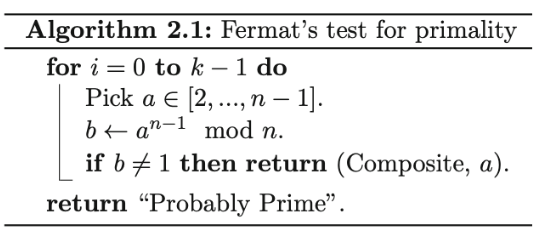
\includegraphics[scale=0.7]{img/fermatprimetest.png}
    \caption{Algorithm for Fermat Primality Test}
\end{figure}

\subsubsection{Miller-Rabin Primality Test}
The Miller-Rabin test is an improvement over the Fermat test. Unlike deterministic primality tests (which can definitively prove whether a number is prime), the Miller-Rabin test provides a result with high probability. If the test declares a number to be composite, then it is definitely not prime. However, if the test declares the number to be prime, there is still a small chance that it is actually composite (this is the ``probabilistic" part). The Miller-Rabin test checks whether a number $n$ passes certain conditions that hold for all prime numbers. It does this by examining the modular arithmetic properties of numbers related to $n$. If $n$ passes these tests, it is likely prime. If it fails, $n$ is definitely composite.

\begin{figure}[h!]
    \centering
    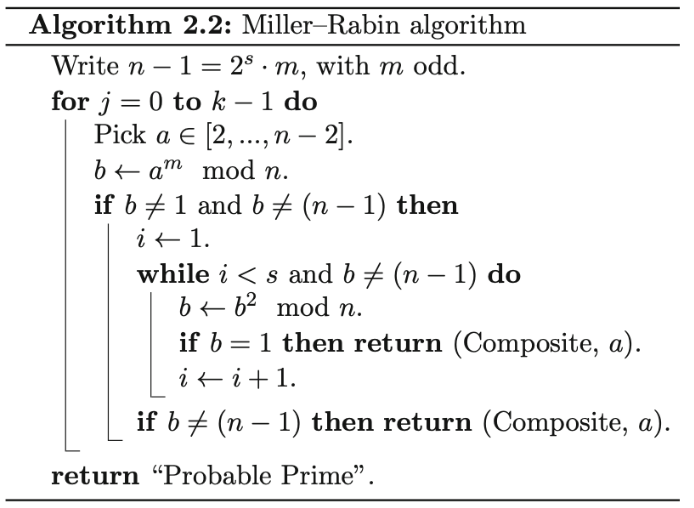
\includegraphics[scale=0.65]{img/MRprimetest.png}
    \caption{Algorithm for Miller-Rabin Test}
\end{figure}

% \begin{enumerate}
%     \item \textbf{Express \( n-1 \) as \( 2^s \cdot d \):}
%     \begin{itemize}
%         \item First, express \( n-1 \) as a product of a power of 2 and an odd integer. Specifically, find \( s \) and \( d \) such that:
%         \[
%         n-1 = 2^s \cdot d, \quad \text{where} \quad d \text{ is odd}.
%         \]
%         \item This can be done by repeatedly dividing \( n-1 \) by 2 until \( d \) becomes odd.
%     \end{itemize}

%     \item \textbf{Choose a random base \( a \):}
%     \begin{itemize}
%         \item Select a random integer \( a \) such that \( 1 < a < n-1 \).
%     \end{itemize}

%     \item \textbf{Compute \( a^d \mod n \):}
%     \begin{itemize}
%         \item Calculate \( a^d \mod n \) using modular exponentiation.
%     \end{itemize}

%     \item \textbf{Check the first condition:}
%     \begin{itemize}
%         \item If \( a^d \equiv 1 \pmod{n} \) or \( a^d \equiv n-1 \pmod{n} \), then \( n \) passes this round of the test.
%     \end{itemize}

%     \item \textbf{Iterate and square:}
%     \begin{itemize}
%         \item If neither of the above conditions hold, square \( a^d \mod n \) repeatedly \( s \) times (i.e., compute \( a^{2^i \cdot d} \mod n \) for \( i = 1, 2, \ldots, s-1 \)).
%         \item Check if any of these intermediate results equals \( n-1 \). If you find \( a^{2^i \cdot d} \equiv n-1 \pmod{n} \) for some \( i \), then \( n \) passes this round.
%     \end{itemize}

%     \item \textbf{Final check:}
%     \begin{itemize}
%         \item If \( n \) does not satisfy the conditions at any stage (i.e., if \( a^{2^i \cdot d} \mod n \neq 1 \) and \( a^{2^i \cdot d} \mod n \neq n-1 \) for all \( i \)), then \( n \) is composite.
%     \end{itemize}

%     \item \textbf{Repeat:}
%     \begin{itemize}
%         \item Repeat steps 2-6 with different random bases \( a \). Each round of testing reduces the probability of error.
%     \end{itemize}
% \end{enumerate}

\subsection{Elliptic Curves}
\begin{defn}
    An elliptic curve is an equation of the form $F: y^2 = x^3 + ax + b \mod p$, with constants a, b.
    \begin{itemize}
        \item $p > 3$, otherwise $x^3 = x$
        \item If P is on F, then also $P + P, P+P+P,$ ... are on F.
    \end{itemize}
\end{defn}

Not all equations make good elliptic curves. They must satisfy a condition that ensures there are no sharp points or self-intersections. The curve must be \emph{smooth} and \emph{non-singular}.
\[ 4a^3 + 27b^2 \neq 0 \]

\textbf{Point Addition:} 
\begin{itemize}
    \item Addition of two points $P$ and $Q$ on the curve gives you another point $R$, which is also on the curve. 
            To add \( P = (x_1, y_1) \) and \( Q = (x_2, y_2) \):
            \begin{enumerate}
                \item Draw a straight line through \( P \) and \( Q \). This line will generally intersect the curve at exactly one more point, say \( R' \).
                \item Reflect \( R' \) across the x-axis to get \( R = (x_3, y_3) \), the result of \( P + Q \).
            \end{enumerate}
            The formulas to compute \( R = (x_3, y_3) \) are:
            \[
            x_3 = \lambda^2 - x_1 - x_2
            \]
            \[
            y_3 = \lambda(x_1 - x_3) - y_1
            \]
            where \( \lambda \) (the slope of the line) is:
            \[
            \lambda = \frac{y_2 - y_1}{x_2 - x_1}
            \]
    \item If you’re adding $P$ to itself (doubling), the line you draw is the tangent to the curve at $P$.
    The formulas for \( R = 2P = (x_3, y_3) \) are:
    \[
    x_3 = \lambda^2 - 2x_1
    \]
    \[
    y_3 = \lambda(x_1 - x_3) - y_1
    \]
    Here, \( \lambda \) (the slope of the tangent) is:
    \[
    \lambda = \frac{3x_1^2 + a}{2y_1}
    \]
    \item If \( P \) and \( Q \) are vertical opposites (e.g., \( P = (x, y) \) and \( Q = (x, -y) \)), the line through them is vertical, and their sum is the \textbf{point at infinity}, \( \mathcal{O} \). Think of \( \mathcal{O} \) as the "zero" for point addition.
    \item Special properties:
    \begin{itemize}
        \item \textbf{Commutative:} \( P + Q = Q + P \)
        \item \textbf{Associative:} \( (P + Q) + R = P + (Q + R) \)
        \item \textbf{Identity Element:} Adding the point at infinity \( \mathcal{O} \) to any point \( P \) gives \( P \) (like adding zero).
    \end{itemize}
\end{itemize}

\begin{figure}[h!]
    \centering    
    \begin{subfigure}[b]{0.3\textwidth}
        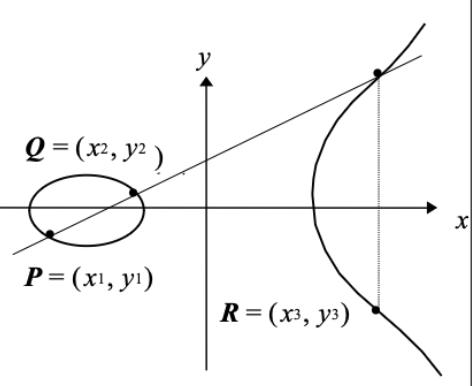
\includegraphics[width=\linewidth]{img/ecadd.png}
        \caption{Point Addition}
    \end{subfigure}
    \hfill
    \begin{subfigure}[b]{0.3\textwidth}
        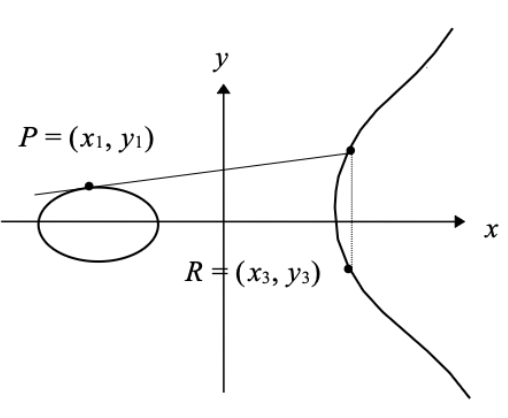
\includegraphics[width=\linewidth]{img/pointdoubling.png}
        \caption{Point Doubling}
    \end{subfigure}
    \hfill
    \begin{subfigure}[b]{0.3\textwidth}
        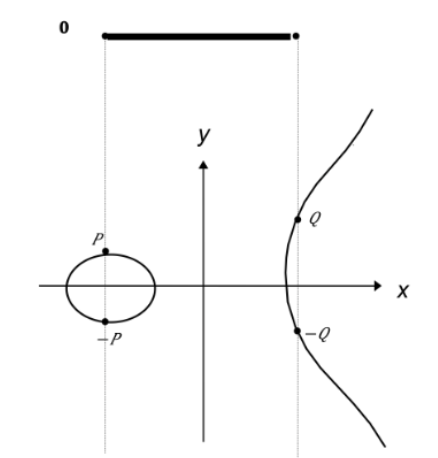
\includegraphics[width=\linewidth]{img/zeropoint.png}
        \caption{Zero Point}
    \end{subfigure}
\end{figure}

Using elliptic curves lets us create very secure systems with shorter keys (really large prime numbers are not required), which means faster and more lightweight encryption.

\begin{defn}
    \textbf{Elliptic Curve Discrete Log Problem}: For a given integer m and a point P, it is easy to compute $Q = mP$. However, given P and Q, it is hard to compute m.
\end{defn}

Imagine a simple operation: start at one point on the curve, "add" it to itself repeatedly, and you get another point. If I tell you the starting point and the number of additions, it's easy to figure out the end point. But if I give you the end point and ask you to figure out the number of additions, that's really hard. This is what makes elliptic curve cryptography (ECC) secure.

\newpage

\section{Lecture 3}

\subsection{The Syntax of Encryption}

\subsection{Classical Ciphers}

\subsubsection{Caesar Cipher}

\subsubsection{Shift Cipher}

\subsubsection{Substitution Cipher}

\subsubsection{Vigenère Cipher}

\subsubsection{Permutation Cipher}


\newpage

\section{Lecture 4}

\subsection{Security Definitions}
\begin{defn}
    Computationally Secure: it takes N operations using the \textbf{best known algorithm} to break a crytographic system and N is too large to be feasible.
\end{defn}

\begin{defn}
    Provably Secure: breaking the system is reduced to solving some well-studied hard problem.
\end{defn}

\begin{defn}
    Unconditional Secure/Perfectly Secure: the system is secure against an adversary with unlimited computational power.
\end{defn}

Key size is important. Advances in computer hardware and algorithms are important. In the future, it will be broken due to hardware or better algorithms.

\subsection{Probability and Ciphers}

\begin{defn}
Let $P$ denote the set of plaintexts, $K$ the set of keys, and $C$ denote the set of cipher texts. $p(P=m)$ is the probability that the plaintext is $m$. Then,
\[
p(C=c) = \sum_{k: c\in \mathbb{C}(k)} p(K=k)\cdot p(P=d_k(c))
\]
\end{defn}

\Comment{add examples in here}

\subsection{Perfect Secrecy}
Previously, the ciphertext revelas a lot of information about the plaintext. We want a system in which ciphertext does not reveal anything about the plaintext. 

\begin{defn}
    Perfect secrecy: a cryptosystem has perfect secrecy if \[ p(P=m | C=c) = p(P=m) \] for all plain texts $m$ and ciphertexts $c$.
\end{defn}

\begin{lem}
    Assume the cryptosystem is perfectly secure, then 
    \[ \#K \geq \#C \geq \#P\] where $\#$ denotes the number of items in the corresponding set. 
\end{lem}

\subsection{One-Time Pad}

\begin{thm}
    Shannon's Theorem: Let $(P, C, K, e_k(), d_k())$ denote a cryptosystem with \( \#K = \#C = \#P\). Then the cryptosystem provides perfect secrecy if and only if:
    \begin{itemize}
        \item Every key is used with equal probability $1/\#K$
        \item For each $m \in P$ and $c \in C$, there is a unique key $k$ such that $c = e_k(m)$
    \end{itemize}
\end{thm}

\Comment{Add modified shift cipher here}

\subsection{Entropy}
Due to the key distribution problem (the key must be as long as the message), perfect secrecy is not practical. Instead, we need a cryptosystem in which \textbf{one key can be used many times}, and \textbf{a  small key can encrypt a long message}. Such a system is not perfectly secure, but it should be computationally secure. We need to measure the amount of informatiomn first: Shannon's entropy. \\

\textbf{Example:} For a specific question X: ``Will you go out with me?'', the answer is Yes or No. If you always say No, the amount of information, $H(X) = 0$. If you always say Yes, $H(X) = 0$. You know the result. If you say Yes and No with equal probability, $H(X) = 1$. When you get the answer, no matter what it is, you learn a lot. Here, $H()$ is the entropy, and is independent of the length of $X$.

\begin{defn}
    Shannon's Entropy: Let $X$ be a random variable which takes a finite set of values $x_i$, with $1 \leq 1 \leq n$, and has a probability distribution $p(x)$. We use the convention that if $p_i = 0$ then $p_i \log_2(p_i) = 0$. The entropy of $X$ is defined as:

    \[ H(X) = -\sum_{i=1}^n p_i \cdot \log_2 p_i\] 

    Properties:
    \begin{itemize}
        \item $H(X) \geq 0$
        \item $H(X) = 0$ if $p_i = 1$ and $p_j = 0$ for $i \neq j$
        \item if $p_i = 1/n$ for all $i$, then $H(X) = \log_2(n)$
    \end{itemize}
\end{defn}

\subsection{Spurious Keys and Unicity Distance}


\newpage

\section{Lecture 5}

\subsubsection{What does it mean to be secure?}
Modern cryptography is focused on three key aspects:
\begin{enumerate}
\item \textbf{Definitions:} Concrete mathematical definition of what it means for a particular cryptographic mechanism to be secure.
\item \textbf{Schemes:} Design the schemes which will (hopefully) meet the security definitions.
\item \textbf{Proofs:} Check whether the design meets the security definitions (provable/reductionist security).
\end{enumerate}

For instance with factorization, given a large number, it is very difficult to factorize. An algorithm to do this efficiently in polynomial time would break all schemes that rely on factorization. 

\subsection{Security Games}
\textbf{Security games} are mathematical frameworks used in cryptography to formally evaluate the security of a computational problem or cryptographic system. They involve an interaction between two entities:

\begin{itemize}
    \item \textbf{The challenger}, who provides an input (e.g., a computational problem).
    \item \textbf{The adversary} (A), who attempts to solve the problem or break the cryptographic system under specific rules and constraints.
\end{itemize}

The goal is to quantify the probability of the adversary's success within a defined resource limit (like time or computational power).

\subsubsection{The FACTOR Problem}
In this example, the security game focuses on the \textbf{Factorization Problem}, where the adversary tries to factorize a large number \(N\), generated as the product of two large primes \(p\) and \(q\). \\

\textbf{Steps in the Security Game:}

\begin{enumerate}
    \item Setup by the Challenger:
    \begin{itemize}
        \item Two large primes \(p\) and \(q\) are randomly chosen, each with a bit size of \(v/2\).
        \item The product \(N = p \cdot q\) is computed and given to the adversary \(A\).
    \end{itemize}
    
    \item Goal of the Adversary:
    \begin{itemize}
        \item The adversary \(A\) ``wins'' the game if they can find two integers \(p'\) and \(q'\) such that:
        \begin{align*}
            p' \cdot q' &= N, \\
            p', q' &\neq p, q.
        \end{align*}
    \end{itemize}

    \item Time Constraint:
    \begin{itemize}
        \item The adversary has a limited amount of computational time \(t\) to solve the problem.
    \end{itemize}
\end{enumerate}

\begin{figure}[h!]
    \centering
    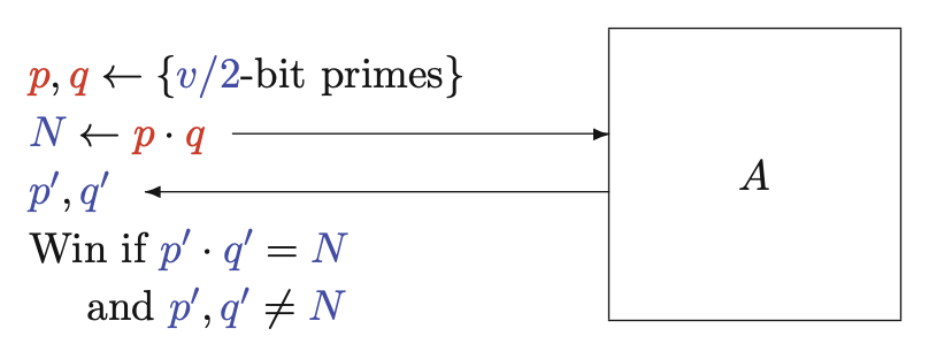
\includegraphics[scale=0.5]{img/game-factor.png}
    \caption{Security game to define the FACTOR problem}
\end{figure}

\subsubsection{Measuring the Adversary's Advantage}

The advantage of the adversary \(A\) in this game is defined as:
\[
\text{Adv}_v^X(A, t) = \Pr\big[A \text{ wins the game } X \text{ for } v = \log_2 N \text{ in time less than } t\big].
\]
Here:
\begin{itemize}
    \item \(v\) is the bit-length of \(N\), representing the problem's complexity.
    \item \(t\) is the allowed time for \(A\).
    \item \(\Pr\) is the probability that \(A\) successfully factors \(N\) under these conditions.
\end{itemize}

\[
\text{Adv}_v^X(A) = 2 \cdot \left| \Pr\big[ A \text{ wins } X \text{ for } v = \log_2 N \big] - \frac{1}{2} \right|
\]
A always wins: 1. A always guesses: 0.

\subsection{Pseudo-Random Functions}
\begin{defn}
A pseudorandom function $F_k(x)$ is a deterministic function that takes an input $x$ and produces an output that is computationally indistinguishable from a truly random function, given only oracle access to the function. No efficient adversary can distinguish between $F_k(x)$ and a truly random function, without knowing the secret key $k$. 
\end{defn}

\textbf{Example in Security Game:}
The game below does not follow Kerkhoff's principle. The adversary always wins, because everything is known. There is no key/security parameter. The adversary can easily check if $F(x) = y$.
\begin{figure}[h!]
    \centering
    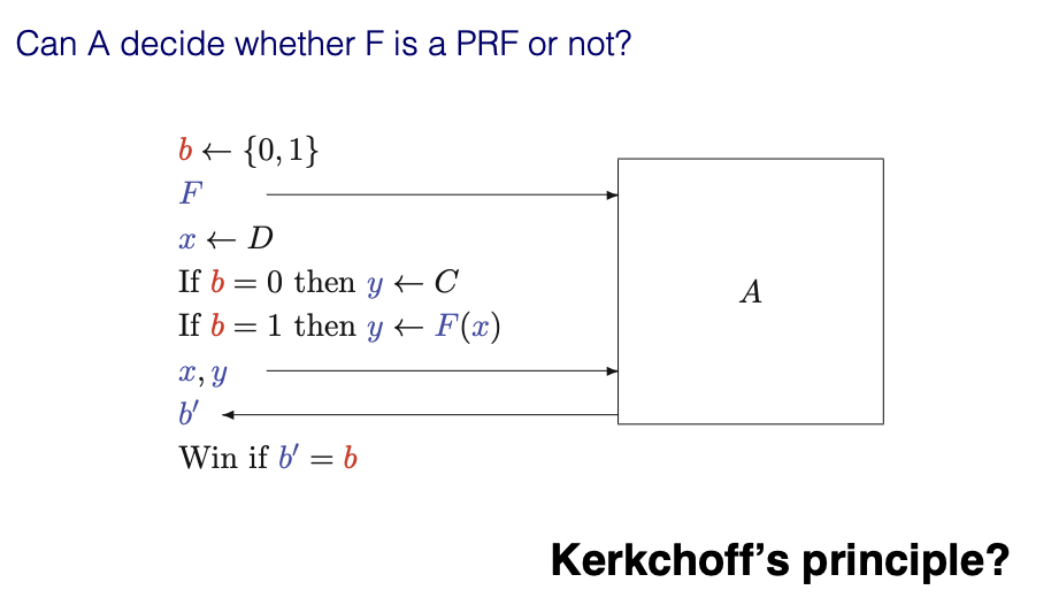
\includegraphics[scale=0.5]{img/PRFbad.png}
    \caption{Security game to define the PRF problem. Here, the adversary always wins!}
\end{figure}

Changing the SG to include a key parameter $k$: we are not having one function $F$, but several functions chosen based on a secret key: $F_k(x)$. The adversary does not know the key. The adversary now has access to an oracle: 

\begin{defn}
An \textbf{oracle} is an abstract, theoretical concept representing a "black box" that provides answers to specific queries according to a defined rule or function. The term is often used to model adversaries' access to resources or information in a controlled manner during security analyses.
\begin{itemize}
    \item The oracle operates according to predefined rules or a specific function (e.g., encryption, decryption, signature generation, or random sampling).
    \item The adversary can query the oracle to obtain information or perform operations, but cannot directly access the oracle's internal workings.
    \item For example, an encryption oracle takes a plaintext as input and outputs the corresponding ciphertext, while a decryption oracle does the reverse.
\end{itemize}
\end{defn}

\begin{figure}[h!]
    \centering
    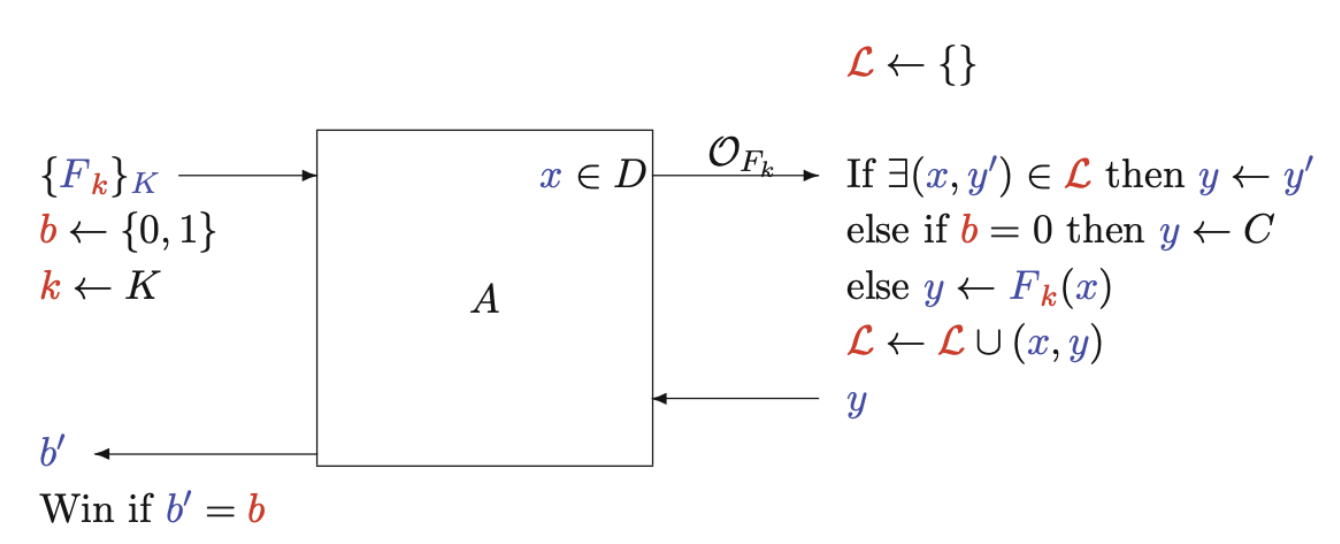
\includegraphics[scale=0.5]{img/PRFfinal.png}
    \caption{The final security game for a PRF}
    \label{PRFfinal}
\end{figure}

\newpage
\textbf{Example: Oracle in a Security Game}
For a PRF function security game, the oracle $\mathcal{O}_k(x)$ behaves as follows:
\begin{itemize}
    \item With secret key $k$, the oracle implements $\mathcal{O}_{F_k}$, where $F_k$ is a pseudorandom function.
    \item Alternatively, the oracle can implement $\mathcal{O}_R$, where $R$ is a truly random function.
    \item The oracle should not give two different answers for the same input $x$. Hence, it has a memory $\mathcal{L}$.
\end{itemize}

The adversary queries the oracle with different $x$ values and observes the outputs. The adversary's goal is to distinguish whether the oracle is implementing a PRF or truly random function, without knowing the secret key $k$. In figure \ref{PRFfinal}, this is indicated by the bit $b$. The adversary wins if they can correctly guess $b$.

\subsubsection{Adversary's Advantage}

The adversary's \textit{advantage} measures how well it can distinguish the oracle's behavior from random guessing. This is formally defined as:

\[
\text{Adv}_{\{F_k\}_K}^{\text{PRF}}(A) = 2 \cdot \left| \Pr\big[A^{O_{F_k}} \text{ wins}\big] - \frac{1}{2} \right|
\]

Key Components:
\begin{itemize}
    \item \( \Pr\big[A^{O_{F_k}} \text{ wins}\big] \): The probability that \( A \) correctly guesses the bit \( b \).
    \item \( \frac{1}{2} \): The probability of guessing \( b \) purely at random.
\end{itemize}

Interpretation:
\begin{itemize}
    \item If \( A \) cannot distinguish \( F_k(x) \) from a random function, its success probability is \( \frac{1}{2} \), meaning \( \text{Adv}_{\{F_k\}_K}^{\text{PRF}}(A) = 0 \).
    \item If \( A \) has some advantage in distinguishing \( F_k(x) \) from random, the value \( \text{Adv} \) increases, indicating the weakness of the PRF.
\end{itemize}

\subsubsection{Why is this important?}
This security game is critical for evaluating whether a function $F_k(x)$ behaves indistinguishably from a truly random function. In cryptographic systems:
\begin{itemize}
    \item Strong PRFs ensure adversaries can't predict outputs or distinguish the function, which is vital for the security of encryption, key derivation, and other cryptographic primitives.
    \item A PRF that is distinguishable from random may leak information or fail to provide the desired security guarantees.
\end{itemize}

\newpage

\subsection{Trapdoor Functions}

\begin{defn}
    A \textbf{one-way function} is a function that is easy to compute in one direction but \emph{hard to invert}.

\begin{itemize}
    \item \textbf{Easy to compute:} Given an input \( x \), it is computationally efficient to calculate \( f(x) \).
    \item \textbf{Hard to invert:} Given \( f(x) \), it is computationally infeasible to find \( x \) (or any \( x' \) such that \( f(x') = f(x) \)) without additional information.
\end{itemize}
\end{defn}

\begin{defn}
    A \textbf{trapdoor} function is a one-way function that is easy to compute in one direction but hard to invert unless a secret "trapdoor" is known. An extra piece of information helps to invert the function, e.g. RSA.
\end{defn}

\begin{figure}[h!]
    \centering
    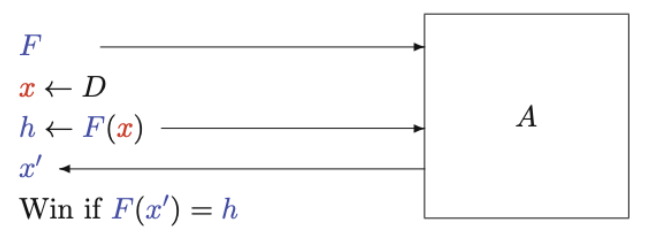
\includegraphics[scale=0.5]{img/OWgame.png}
    \caption{Security game for a one-way function}
    \label{trapdoor}
\end{figure}

\subsection{Public Key Cryptography}
\begin{itemize}
    \item \textbf{Key distribution problem} in symmetric (private key) systems.
    \item A \textbf{key pair} is needed:
    \begin{itemize}
        \item \textbf{Private key} for decryption (only the owner can decrypt).
        \item \textbf{Public key} for encryption (everyone can encrypt).
    \end{itemize}
    \item Public and private keys are linked in a mathematical way:
    \begin{itemize}
        \item Obtaining the private key from the public key is \textbf{NOT easy}.
        \item Obtaining the public key from the private key is \textbf{easy}.
    \end{itemize}
\end{itemize}

The security of an encryption scheme (both symmetric and asymmetric) is dependent on:
\begin{itemize}
    \item The goal of the adversary
    \item The types of attacks allowed
    \item The computational model
\end{itemize}

\subsection{Basic Notions of Security}
Notation and valid encryption: 
\[ \forall k \in \mathbb{K}, \forall m \in \mathbb{P}, d_k(e_k(m)) = m \]
What does it mean for a symmetric encryption scheme to be secure? Adversary should not learn the underlying (plaintext) message.

\subsubsection{OW-PASS attack}
One-wayness under passive attack.
\begin{itemize}
    \item Adversary's Capability: The adversary only observes the encryption of a plaintext message but cannot interact with the encryption mechanism in any way.
    \item Goal: The adversary is given the ciphertext \( c = \text{Enc}(m) \) and attempts to recover the plaintext \( m \).
    \item Assumptions:
    \begin{itemize}
        \item The adversary has no control over the plaintexts being encrypted.
        \item Security is evaluated against passive observers who can only eavesdrop.
    \end{itemize}
    \item Use Case: Suitable for scenarios where the attacker does not have active access to the encryption process.
\end{itemize}

\begin{figure}[h!]
    \centering
    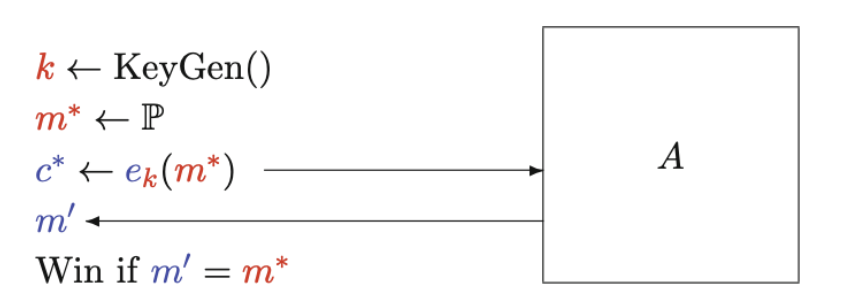
\includegraphics[scale=0.5]{img/OWpass.png}
    \caption{Security game for symmetric key OW-PASS}
\end{figure}


\subsubsection{OW-CPA attack}
OW-PASS is very limiting for the adversary. She should have an encryption oracle. One-Wayness under Chosen Plaintext Attack:
\begin{itemize}
    \item Adversary's Capability: The adversary can interact with the encryption mechanism by choosing plaintexts and obtaining their corresponding ciphertexts.
    \item Goal: The adversary, after observing ciphertexts for chosen plaintexts, attempts to recover the plaintext of a given ciphertext.
    \item Assumptions:
    \begin{itemize}
        \item The adversary can actively query the encryption oracle with plaintexts of their choice.
        \item This security definition is stronger than OW-PA because it assumes a more powerful adversary.
    \end{itemize}
    \item Use Case: Applies to scenarios where the attacker has partial or controlled access to the encryption process, such as in chosen plaintext attacks on public-key cryptography.
\end{itemize}

\begin{figure}[h!]
    \centering
    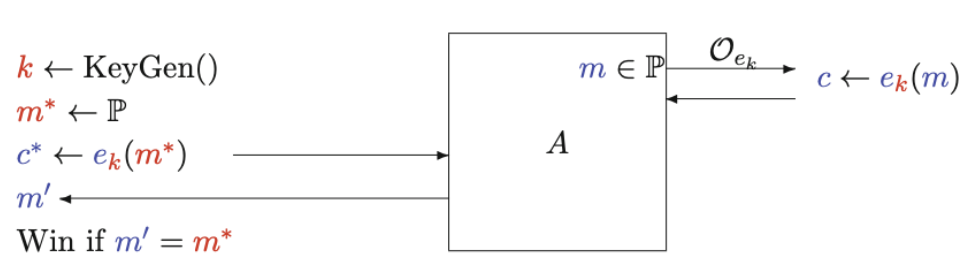
\includegraphics[scale=0.5]{img/OWCPA.png}
    \caption{Security game for symmetric key OW-CPA}
\end{figure}

\subsubsection{OW-CCA attack}
The adversary should be able to decrypt as too (limited number). Thus, One-wayness under Chosen Ciphertext Attack:

\begin{itemize}
    \item Adversary's Capability:
    The adversary is allowed to interact with both the encryption and decryption oracles. Specifically, they can:
    \begin{itemize}
        \item Query the decryption oracle for the decryption of any ciphertext \( c \), except for the target ciphertext \( c^* \).
        \item Query the encryption oracle to obtain the ciphertext for any plaintext \( m \) of their choice.
    \end{itemize}
    
    \item Goal:
    The adversary attempts to recover the plaintext \( m^* \) from a given target ciphertext \( c^* = \text{Enc}(m^*) \).

    \item Assumptions:
    \begin{itemize}
        \item The adversary has powerful capabilities to both query encryption for chosen plaintexts and query decryption for chosen ciphertexts.
        \item The decryption oracle cannot be used directly on the target ciphertext \( c^* \) to prevent trivial success.
    \end{itemize}

    \item Use Case:
    \begin{itemize}
        \item OW-CCA security is crucial for applications requiring strong guarantees against active attackers who can manipulate ciphertexts.
        \item It is relevant in scenarios such as securing communications where adversaries can intercept, modify, and replay ciphertexts.
    \end{itemize}

    \item Key Features:
    \begin{itemize}
        \item Adversary's Advantage: OW-CCA tests the robustness of a cryptographic scheme against the most powerful adversaries who can both observe and manipulate encrypted communications.
        \item Stronger Security: OW-CCA provides stronger guarantees compared to OW-PA and OW-CPA as it accounts for adversaries who have decryption capabilities.
    \end{itemize}
\end{itemize}

\begin{figure}[h!]
    \centering
    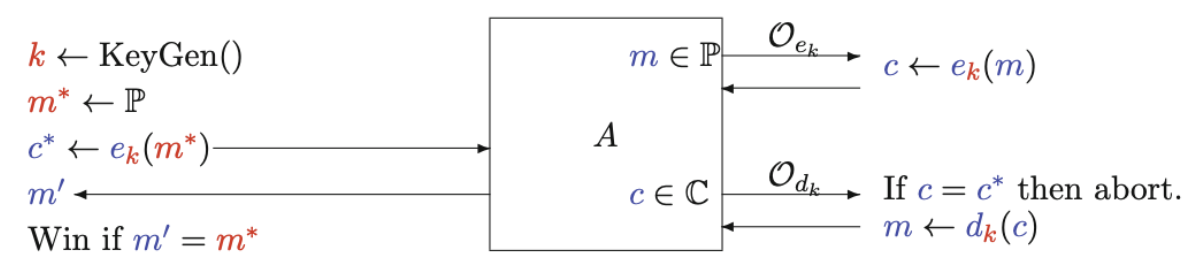
\includegraphics[scale=0.5]{img/OWcca.png}
    \caption{Security game for symmetric key OW-CCA}
\end{figure}

\subsection{Modern Notions of Security}
Before, the attacks assumed that you obtain the whole key. In real life, the adversary can also partially break the system (one bit of the key). The adversary should not be allowed to obtain \textbf{any} information about the plaintext! \\

Perfect secrecy is not practical, because every plaintext needs to have the same probability. To do so, the key needs to be as long as the message.

\begin{defn}
Semantic security: like perfect security but the adversary has polynomially bounded computing power. The adversary cannot extract partial knowledge. 

\[g: M \rightarrow \{0,1\}\] 
\[Pr[g(m) = 1] = Pr[g(m) = 0] = \frac{1}{2}\]
\[ Adv_{\prod}^{\text{SEM}} (S) = 2 \cdot \left| Pr[S(c) = g(d_k(c))] - \frac{1}{2} \right| \]\end{defn}

Semantic security ensures that an adversary cannot learn any meaningful information about a plaintext from its ciphertext, even if they have some prior knowledge about the plaintext. Formally, a cryptosystem is semantically secure if, given a ciphertext, the adversary cannot distinguish between the encryptions of two chosen plaintexts. \\

Semantic security is \emph{difficult to show}! Polynomial security (IND) is easier to show. If a system is IND secure, it is also semantically secure.

\begin{defn}
IND Security: an encryption scheme is \emph{IND-secure} if the ciphertexts of two plaintexts are indistinguishable to an adversary, ensuring that the adversary gains no advantage from observing ciphertexts, even with access to oracles (depending on the attack model).
\end{defn}

IND Security ensures that an adversary cannot distinguish between the ciphertexts of two chosen plaintexts, even if they select the plaintexts themselves. This is a fundamental property of secure encryption. IND Security requires the use of \emph{probabilistic} encryption for public-key encryption schemes to ensure that ciphertexts for the same plaintext look different every time they are encrypted. This randomness prevents adversaries from exploiting patterns in ciphertexts to distinguish between plaintexts.

\subsubsection{IND Security Games} 
The IND framework is defined under different adversarial capabilities: \\

\textbf{IND-CPA} (Indistinguishability under Chosen Plaintext Attack):
\begin{itemize}
    \item The adversary can choose two plaintexts $m_0$ and $m_1$.
    \item A random bit $b$ is chosen, and the ciphertext of $m_b$ is given to the adversary.
    \item The adversary must guess $b$.
    \item Success probability $> \frac{1}{2}$ implies a weakness in the scheme.
\end{itemize}

\textbf{IND-CCA} Indistinguishability under Chosen Ciphertext Attack):
\begin{itemize}
    \item Similar to IND-CPA, but the adversary is also allowed to query a decryption oracle.
    \item The adversary cannot query the decryption oracle for the target ciphertext.
    \item This provides a stronger security guarantee than IND-CPA.
\end{itemize}

\begin{figure}[h!]
    \centering
    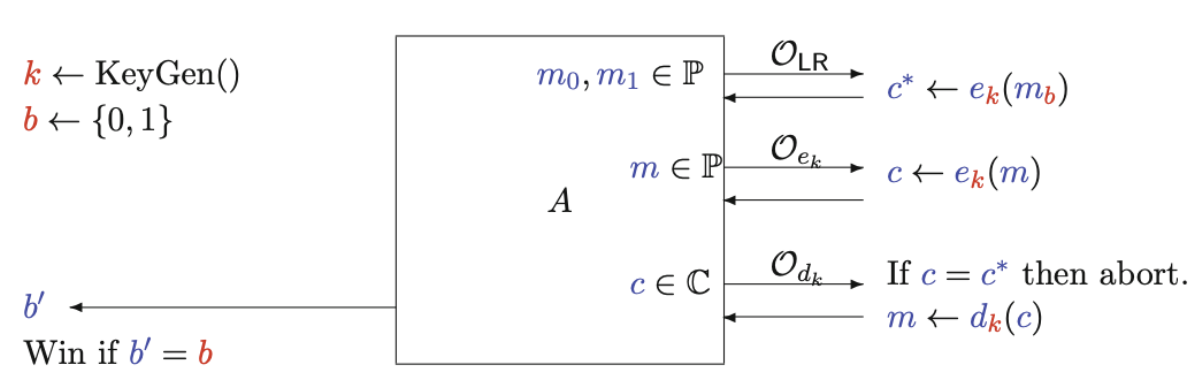
\includegraphics[scale=0.5]{img/INDcca.png}
    \caption{Security game for symmetric key IND-CCA}
    \label{INDcca}
\end{figure}

If the cryptosystem is deterministic, you can fool the oracles. In figure \ref{INDcca}, $\mathcal{O}_{LR}$ will only encrypt one of $m_1, m_2$. You use the other message in the second step $\mathcal{O}_{e_k}$, and check if you receive the same ciphertext as in step 1.
The decryption oracle $\mathcal{O}_{d_k}$ can be fooled if there is a relationship between the plain text and the cypertext. This is possible in homomorphic encryption.
For secure communication, homomorphism is not appreciated. But we have it because in public cryptosystems we rely on mathematically difficult problems.
\begin{defn}
An encryption algorithm is secure if it is semantically secure against a CPA attack.
\end{defn}

\begin{defn}
An encryption algorithm is secure if it is IND-CCA secure.
\end{defn}

\begin{thm}
A system which is IND-PASS secure must be semanticallt secure against passive adversaries.

\[ \prod \text{ is IND-CCA} \Rightarrow \prod \text{ is IND-CPA} \Rightarrow \prod \text{ is IND-PASS} \] 
\[ \prod \text{ is IND-XXX} \Rightarrow \prod \text{ is OW-XXX} \]
\end{thm}

\subsection{Other Notions of Security}
\Comment{Add definitions here from slides}

\subsection{Random Oracle Model}
\Comment{Finish later}

\newpage

\section{Lecture 6}

Randomness is extremely important in cryptography, and the same random values should never be used twice. It is hard to achieve, often we use pseudo-random number generators (PRNGs) to generate randomness. \\

\textbf{Example of Importance of Randomness:}
In a perfect secrecy scheme, the key is as long as the message. If the same key is reused even once, the messages can be decrypted. XORing their ciphertexts effectively removes the key, leaving a direct relationship between the two plaintexts. \\

For a message $m$ and key $k$, the ciphertext is $c = m \oplus k$, where $\oplus$ is the XOR-operation. For two messages encrypted with the same key:

\[c_1 = m_1 \oplus k\] 
\[c_2 = m_2 \oplus k\]

Now, if we XOR the ciphertexts:
\[c_1 \oplus c_2 = (m_1 \oplus k) \oplus (m_2 \oplus k)\]

Using the property of XOR that \(a \oplus a = 0\) and \(a \oplus b \oplus a = b\), we can deduce:

\[
c_1 \oplus c_2 = m_1 \oplus m_2 \oplus k \oplus k
\]

\[
c_1 \oplus c_2 = m_1 \oplus m_2
\]

Thus, the XOR of the two ciphertexts directly reveals the XOR of the two plaintexts. The ``distance" between two messages $m_1$ and $m_2$ represented by their XOR operation $m_1 \oplus m_2$, reveals the bitwise differences between them. This is often inpreted as the Hamming distance (the number of positions at which two strings of the same length differ) between the two messages. The XOR distance not only represents differences but can be exploited to reconstruct messages in insecure systems where the same key is reused (for instance, when the adversary knows one of the plaintexts already and can reconstruct the other).

\subsection{Stream Ciphers}

\begin{defn}
Stream ciphers are based on zeroes and ones. They encrypt bits (bit by bit) instead of blocks of plaintext. Due to bit operations, they are very fast. Easy to implement on hardware and software.
\end{defn}

Consider the following stream cipher:

\[ c = m \oplus F_k(0) \]

Where $F_k(0)$ is a function that generates a keystream based on the key $k$. The keystream is XORed with the plaintext to produce the ciphertext. The keystream is generated by a pseudo-random number generator (PRNG) that takes the key as input. \\

If the key was the same length of the message it would be perfect, but creating such a long key would be very inefficient (only done for government to government communication).
However, we can use a shorter key to mimic this behaviour. The short key is used to choose the output of a PRF (the key is the seed of the PRNG). It will mimic pseudo-randomness long enough (until it repeats itself). The cipher will be passive secure if the PRF is random enough.

\subsection{Linear Feedback Shift Registers (LFSRs)}
We can use LFSRs for generating a binary stream.

\begin{defn}
 A \textbf{Linear Feedback Shift Register} (LFSR) is a sequential shift register that generates a sequence of bits based on a linear feedback function. It consists of:
 \begin{itemize}
    \item A sequence of single-bit registers (0 or 1)
    \item Feedback function: a linear function (usually XOR) that determines how bits are fed back into the register.
    \item Tap positions in the register used in the feedback function.
 \end{itemize}
\end{defn}

\textbf{How it works:}
\begin{enumerate}
    \item Initialization: The register is initialized with a seed value (a non-zero starting state).
    \item Bit Shifting: The register shifts all bits to the right (or left), discarding the last bit.
    \item Feedback Calculation: A new bit is computed based on the XOR of the bits in the ``tapped'' positions.
    \item Repeat: The new bit is inserted into the first position of the register, and the process repeats to generate the next bit in the sequence.
\end{enumerate}

\begin{figure}[h!]
    \centering
    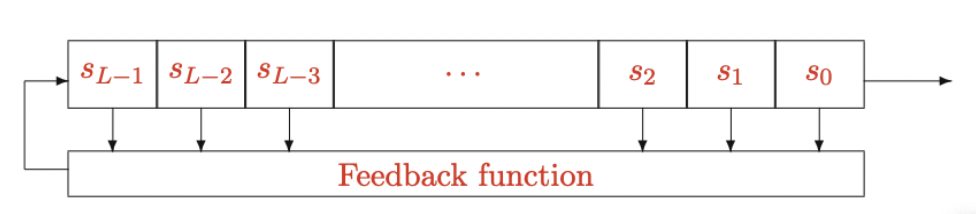
\includegraphics[width=0.5\textwidth]{img/LFSR.png}
    \caption{Feedback shift register}
\end{figure}

The initial state is very important, as it determines the entire sequence (whole sequence of zeroes always results in zeroes). The feedback function and length of the registers are also important.

\subsubsection{Properties of LFSRs}
\begin{itemize}
    \item Periodicity: LFSRs are periodic; they generate a sequence that eventually repeats. The maximum period is $2^n - 1$, where $n$ is the register size, achieved when the feedback taps correspond to a primitive polynomial.
    \item Deterministic: If the initial state (seed) and feedback function are known, the sequence is fully predictable.
    \item Efficiency: LFSRs are computationally efficient, using only shift and XOR operations.
\end{itemize}

\subsubsection{Feedback Functions}
Feedback functions in shift registers are used to compute the new bit that is fed back into the register. The key difference between linear and nonlinear feedback functions lies in how they combine the bits from the register.

\begin{table}[h!]
    \centering
    \renewcommand{\arraystretch}{1.2} % Adjust row spacing
    \begin{tabular}{|>{\raggedright\arraybackslash}m{4cm}|>{\raggedright\arraybackslash}m{5cm}|>{\raggedright\arraybackslash}m{5cm}|}
    \hline
    \textbf{Feature} & \textbf{Linear Feedback} & \textbf{Nonlinear Feedback} \\
    \hline
    \textbf{Operations} & XOR and other linear operations & Nonlinear operations (AND, OR, S-boxes, etc.) \\
    \hline
    \textbf{Predictability} & Easier to predict with known state & Harder to predict, more secure \\
    \hline
    \textbf{Efficiency} & Computationally efficient & More computationally intensive \\
    \hline
    \textbf{Periodicity} & Periodic, with a maximum of $2^n - 1$ & Can be non-periodic or have a very long period \\
    \hline
    \textbf{Applications} & Pseudo-random generators, CRC & Secure encryption, cryptographic systems \\
    \hline
    \end{tabular}
    \caption{Comparison of Linear and Nonlinear Feedback Functions}
    \label{tab:feedback_comparison}
\end{table}

We would like to have a non-linear feedback function, but these are difficult to design. Difficult to estimate whether it is a good non-linear function. When you hit 0 the whole value chain becomes 0, and the cycle is broken. \\

\subsubsection{Zero State in Feedback Functions:}
If an LFSR (or any shift register using feedback functions) reaches the value \textbf{zero}, the system will typically ``lock'' into this state and remain there indefinitely. This is because:

\begin{enumerate}
    \item Feedback Function Output: In a linear feedback system, the XOR of all zeros is zero, meaning that once all bits are zero, the feedback function will continue producing zeros.
    \item State Transition: The state of the LFSR will not change, and the register will stay stuck at zero, generating an output sequence that consists entirely of zeros.
\end{enumerate}

Implications:
\begin{itemize}
    \item \textbf{In LFSRs:}
    \begin{itemize}
        \item The sequence degenerates and loses all pseudo-randomness, becoming a constant stream of zeros.
        \item This reduces the period of the LFSR to just 1, which is undesirable, especially in cryptographic or pseudo-random number generation applications.
    \end{itemize}
    
    \item \textbf{In Cryptographic Systems:}
    \begin{itemize}
        \item If the feedback function hits zero during an encryption or random number generation process, it can render the output insecure.
        \item Attackers can easily exploit the fact that the system produces predictable, non-random output (all zeros).
    \end{itemize}
\end{itemize}

Avoiding the Zero State:
\begin{enumerate}
    \item Seed Initialization: The initial state (seed) of the register is carefully chosen to ensure it is non-zero.
    \item Primitive Polynomials: For LFSRs, the taps (feedback positions) are chosen based on primitive polynomials. This ensures the register cycles through all possible non-zero states ($2^n - 1$) before repeating.
    \item Nonlinear Feedback Functions: Nonlinear systems often include mechanisms to avoid degenerative states like zero, introducing additional complexity to prevent such behavior.
    \item External Checks: Some systems include checks to ensure that a zero state is never reached, restarting the LFSR with a valid non-zero state if necessary.
\end{enumerate}

\subsubsection{Mathematical Expression}
Cell is tapped or not (content of the cell contributes to the feedback function yes or no):
\[
[c_1, c_2, \dots, c_L]
\]

Initial state of the registers:
\[
[s_{L-1}, \dots, s_1, s_0]
\]

Output:
\[
[s_0, s_1, s_2, s_3, \dots, s_{L-1}, s_L, s_{L+1}, \dots]
\]

Then, for \(j \geq L\):
\[
s_j = c_1 \cdot s_{j-1} \oplus c_2 \cdot s_{j-2} \oplus \cdots \oplus c_L \cdot s_{j-L}.
\]

However, we need to see a repetition after a certain period, \(N\), such that:
\[
s_{N+i} = s_i.
\]

\(N\) can be maximum \(2^L - 1\). \\

The \textbf{connection polynomial} $C(X)$ describes how the bits stored in the LFSR are combined to produce the feedback bit, which determines the next state of the LFSR. It is defined as:

\[ C(X) = 1 + c_1 \cdot X + c_2 \cdot X^2 + \dots + c_L \cdot X^L \in \mathbb{F}_2\left[X \right] \]

where $\mathbb{F}_2\left[X \right]$ is the set of polynomials over the binary field (coefficients are either 0 or 1). Proper choice of $C(X)$ can result in a maximal period of $2^L - 1$.\\

The \textbf{characteristic polynomial} $G(X)$ describes the LFSR's output sequence and the polynomial that can be used to generate the entire sequence of output bits. It is a function of the feedback logic defined by the connection polynomial.

\[ G(X) = X^L \cdot C(1/X) \]

\textbf{Example:}

\begin{figure}[h]
    \centering
    \begin{subfigure}{0.45\textwidth}
        \centering
        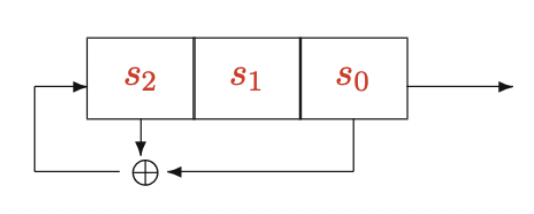
\includegraphics[width=\textwidth]{img/lfsr1.png}
        \caption{$X^3 + X + 1$}
    \end{subfigure}
    \hfill
    \begin{subfigure}{0.45\textwidth}
        \centering
        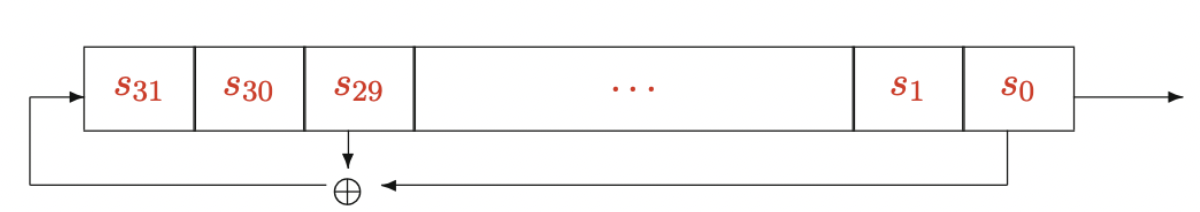
\includegraphics[width=\textwidth]{img/lfsr2.png}
        \caption{$X^{32} + X^3 + X + 1$}
    \end{subfigure}
    \caption{Linear Feedback Shift Register Examples}
    \label{fig:lfsr-examples}
\end{figure}

\begin{itemize}
    \item[a)] This is a small LFSR with length $L=3$, described by the connection polynomial $C(X) = X^3 + X + 1$. There are 3 registers: $s_0, s_1, s_2$. The feedback function involves: $X^3$ (feedback from the last register), $X$ (feedback from the first register), and a constant 1. At each step, the contents of the tapped cells ($s_2, s_0$) are XOR-ed to produce a new bit.
    \item[b)] This is a much larger LFSR with length $L=32$, described by the connection polynomial $C(X) = X^{32} + X^3 + X + 1$. There are 32 registers. The feedback function involves the 32nd (last) register, the 3rd register, the 1st register, and a constant 1. The characteristic polynomial $G(X)$ is used to generate the entire output sequence. \Comment{I dont get the exp values for this one??}
\end{itemize}

Note: The connection polynomial determines which registers contribute to the feedback. But is not a direct description of the output stream itself. Instead, it describes the feedback mechanism of the LFSR. \\

How do we know that the feedback function is a good one, such that we achieve the maximum length before the stream cipher repeats itself?

\subsubsection{Primitive Polynomial}
\begin{defn}
A \emph{primitive polynomial} is a polynomial that generates a maximal-length sequence in a finite field, particularly in the context of binary fields $\mathbb{F}_2$ (i.e., polynomials whose coefficients are either 0 or 1). Specifically, for a polynomial to be \textit{primitive}, it must satisfy the following conditions:

\begin{itemize}
    \item The polynomial must be \textbf{irreducible} over $\mathbb{F}_2$ (i.e., it cannot be factored into the product of lower-degree polynomials with coefficients in $\mathbb{F}_2$).
    \item The polynomial must generate a sequence that cycles through all the nonzero elements of the finite field $\mathbb{F}_{2^L}$, where $L$ is the degree of the polynomial.
\end{itemize}
    
In simpler terms, a primitive polynomial produces a sequence of numbers that goes through all possible states except the zero state (when viewed as an LFSR) before repeating.
\end{defn}

When used in LFSRs, primitive polynomials ensure that the generated sequence has a \emph{maximum length} before it repeats. The length of the sequence is $2^L -1$, where $L$ is the degree of the polynomial.

\begin{thm}
    If N is the period, then the characteristic polynomial $f(x)$ is a factor of $1-X^N$. 
\end{thm}


\[ C(X) = 1 + c_1 \cdot X + c_2 \cdot X^2 + \dots + c_L \cdot X^L \in \mathbb{F}_2\left[X \right] \]

Conditions for $C(X)$:
\begin{itemize}
    \item The highest coefficient $c_L$ = 0: the polynomial is singular. This means that $C(X)$ is not a full degree of $L$ and cannot properly generate sequences of maximal length in an LFSR.
    \item The highest coefficient $c_L$ = 1: the polynomial is non-singular. $C(X)$ is a full degree of $L$ and there is a periodicity in the sequences generated by the polynomial. The behaviour of the sequence depends on whether $C(X)$ is irreducible or not.
\end{itemize}

$C(X)$ is irreducible if it cannot be factored into smaller polynomials over $\mathbb{F}_2\left[X \right]$ (other than itself and 1).
Then, the period of the sequence generated by the LFSR is the \emph{smallest} N such that $C(X)$ divides $1 + X^N$.
$N$ will satisfy $N | (2^L-1)$. \\

\textbf{Example:}
3 registers, maximum length is 7:
\[m = 3, p = 2^3 -1 = 7\] 
So we need to find the factors of:
\[1 - x^y = (1-x)(1 + x + x^3)(1 + x^2 + x^3)\]

The divisors of this polynomial (irreducible polynomials) will have a period of 7.

\subsection{Period}

The presence of disjoint cycles in an LFSR, such as in figure \ref{fig:lfsr-period}, has implications for randomness:

\begin{figure}[h]
    \centering
    \begin{subfigure}{0.45\textwidth}
        \centering
        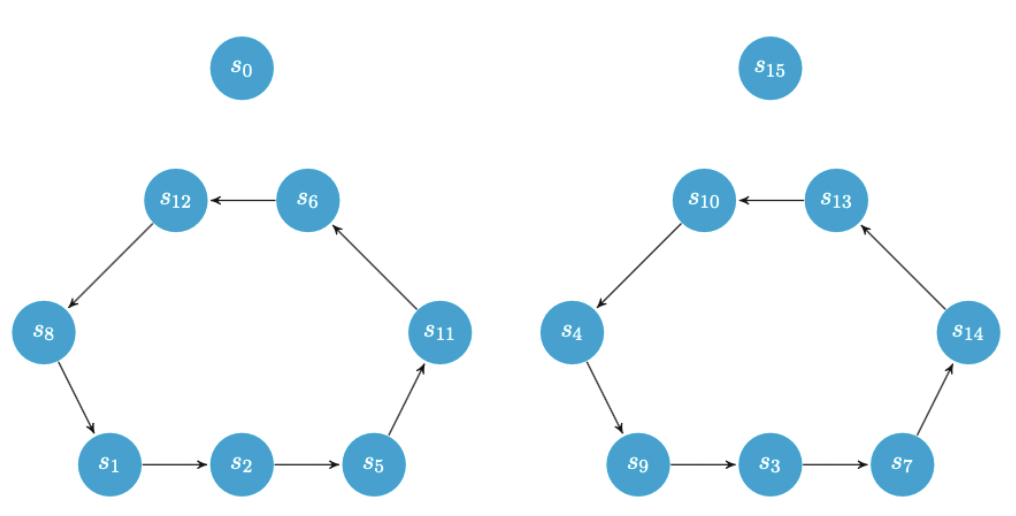
\includegraphics[width=\textwidth]{img/lfsrperiod1.png}
        \caption{$X^4+X^3 + X^2 + 1$}
    \end{subfigure}
    \hfill
    \begin{subfigure}{0.45\textwidth}
        \centering
        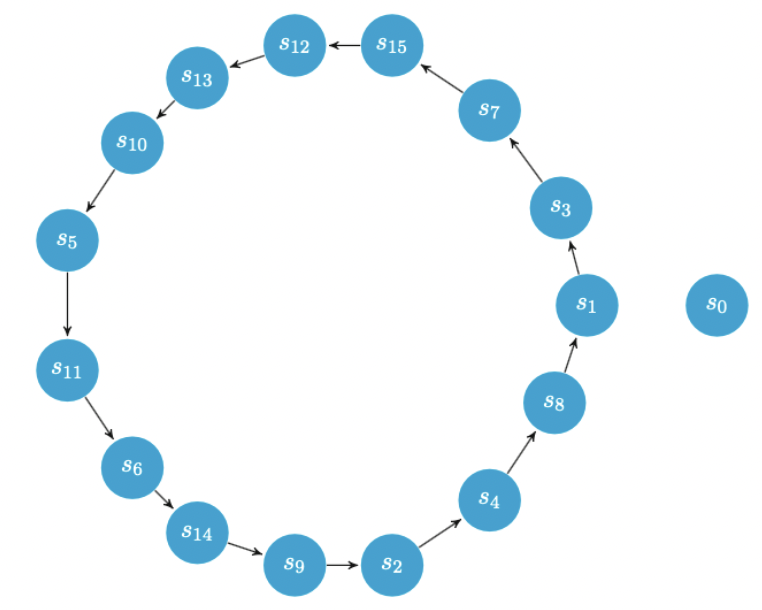
\includegraphics[width=\textwidth]{img/lfsrperiod2.png}
        \caption{$X^4 + X + 1$}
    \end{subfigure}
    \caption{State transitions of 4-bit LFSRs with connection polynomials}
    \label{fig:lfsr-period}
\end{figure}

\begin{itemize}
    \item The output sequence splits into two disjoint cycles of length 7 instead of a single cycle of length \( 2^L - 1 \) (15 for \( L = 4 \)).
    \item Reduced Period: The sequence repeats earlier, reducing the overall period and uniformity.
    \item Loss of Randomness: Missing states lead to gaps, making the sequence predictable and non-random.
    \item Cause: The connection polynomial is \textit{not primitive}, preventing the LFSR from achieving a maximum-length sequence.
\end{itemize}

The right polynomial results in a big cycle with all states included, except for the zero state, as expected.

\subsection{Security of LFSRs}
With $L$ registers and $2L$ known output bits, the connection polynomial can be revealed. It is a linear system. If you have sufficient equations, you can solve the linear system.
\begin{itemize}
    \item First $L$ bits reveal the $s$ values
    \item We need to learn $L$ unknowns: $c$ values
\end{itemize}

\[ s_j = \sum^L_{i=1} c_i \cdot s_{j-i} \pmod{2} \]

Therefore, LFSRs are not secure!

\Comment{Linear complexity notes here}

\subsection{Combining LFSRs}
LFSR-based stream ciphers are very fast ciphers, suitable for implementation in hardware, to encrypt real-time data such as voice or video. But they need to be augmented with a method to produce a form of non-linear output.

Create fast and secure non-linear behaviour by combining multiple LFSRs into a non-linear combination function: 

\begin{figure}[h!]
    \centering
    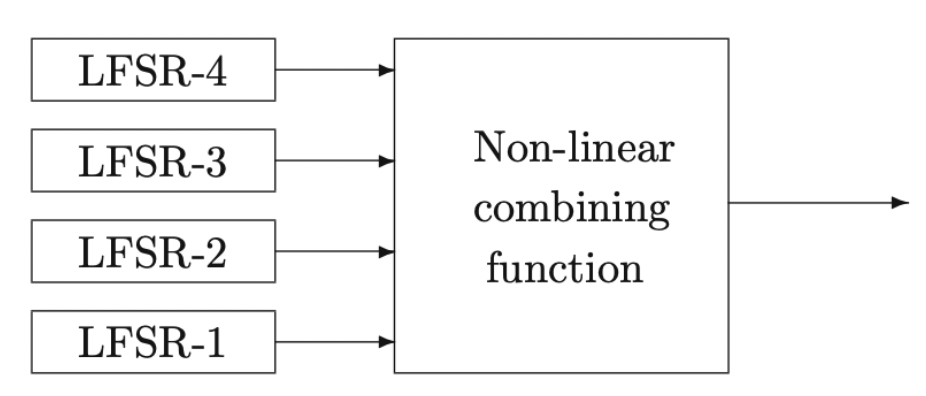
\includegraphics[width=0.5\textwidth]{img/combinelfsr.png}
    \caption{Combining LFSRs}
\end{figure}

\subsubsection{Non-linear Combiners}
Examples covered in lecture are:
\begin{itemize}
    \item Alternating-step generator
    \item Shrinking generator
    \item A5/1
    \item Trivium
    \item RC4
\end{itemize}
\Comment{How much do we need to know about these?}

\newpage

\section{Lecture 7}

Two families: symmetric cryptosystems use the same key for encryption and decryption. They rely on the principles from classical systems: substitution, permutation, and transposition. The reversing operation is dependent on the key.
Asymmetric cryptosystems, on the other hand, use a pair of mathematically related keys—one for encryption (public key) and another for decryption (private key)—relying on complex mathematical problems for security.

\subsection{Block Ciphers}
\begin{defn}
A \textbf{block cipher} is a deterministic cryptographic algorithm that operates on fixed-size blocks of data, typically \( n \) bits, using a symmetric key to perform encryption or decryption. It transforms a plaintext block of size \( n \) bits into a ciphertext block of the same size through a series of reversible, structured operations, and vice versa.

\end{defn}
\begin{figure}[h!]
    \centering
    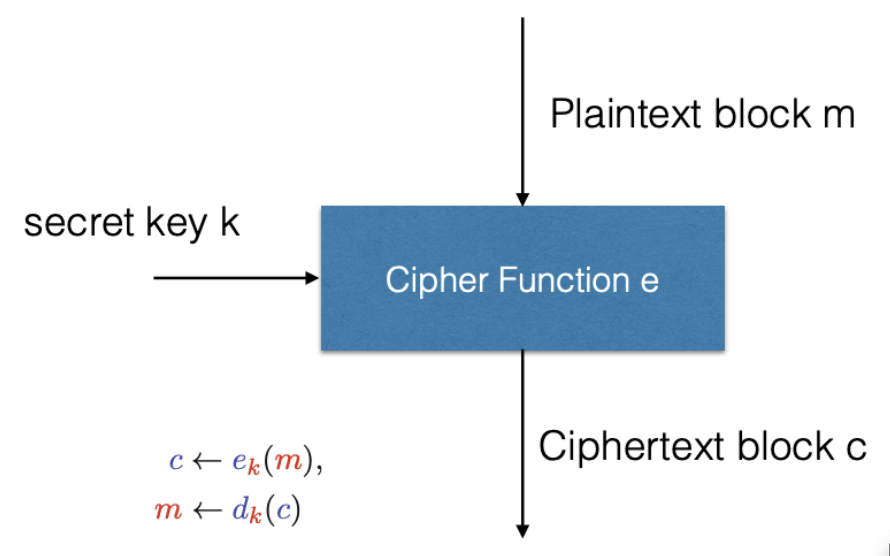
\includegraphics[width=0.5\textwidth]{img/blockcipher.png}
    \caption{Block Cipher}
    \label{fig:block_cipher}
\end{figure}

where
\begin{itemize}
    \item $m \in \{0,1\}^n$ is the plaintext block,
    \item $k \in K$ is the secret key, chosen from key space K,
    \item $e$ is the encryption function,
    \item $d$ is the decryption function,
    \item $c \in \{0,1\}^b$ is the ciphertext block.
\end{itemize}

NOTE: Block ciphers are not proper encryption schemes. You need to combine them with modes of operation! Otherwise your system will not be secure.

\subsubsection{Properties of Block Ciphers}
\begin{enumerate}
    \item Input data block: Plaintext is divided into equal-sized blocks.
    \item Encryption/Decryption: Each block undergoes multiple transformations (substitution, permutation, and mixing) to produce ciphertext.
    \item Key: A symmetric key is applied in multiple \emph{rounds} to ensure security.
    \item Padding: If the last block of plaintext is smaller than the block size, padding is added.
    \item Modes of operation: Block ciphers work with data larger than one block by using modes like:
    \begin{itemize}
        \item ECB (Electronic Codebook)
        \item CBC (Cipher Block Chaining)
        \item GCM (Galois/Counter Mode)
    \end{itemize}
\end{enumerate}
Block ciphers are typically \emph{64 bits} (in DES), \emph{128 bits} (in AES) or more (in modern ciphers). They should act like a \emph{pseudorandom permutation} (PRP).

\begin{defn}
A \textbf{pseudorandom permutation} (PRP) is a function that defines a bijective (one-to-one and onto) mapping between input and output spaces, such that it is computationally indistinguishable from a truly random permutation when the key is unknown. 
\end{defn}

In order to limit the advantage of the adversary, the key space is kept very large (e.g. $Adv \ 1/|K|$). A block cipher is a \emph{building block} for designing a cipher (a PRP). A block cipher with a \emph{Mode of Operation} is a cipher. The goal is to design an IND-CCA secure cipher.

\subsubsection{Design}
DES and AES are iterated block ciphers. They \emph{repeat a simple round function}. The round $r$ can be fixed or variable. The more rounds, the higher the security of the cipher.
\begin{itemize}
    \item In each round, a round key, derived from the key $k$, is used (by key scheduling algorithm) to process a block
    \item The round function should be \emph{invertible}; for decryption the round keys are used in reverse order
    \item In DES: the round is invertible but not the round function
    \item In AES: both the round and the round function are invertible
\end{itemize}

\begin{defn}
    The \textbf{confusion-diffusion} paradigm is a fundamental design principle for secure cryptographic systems, particularly block ciphers.
    \begin{itemize}
        \item \textbf{Confusion:} Confusion ensures that the relationship between the key and the ciphertext is highly complex, making it difficult for an attacker to infer the key, even if they have access to multiple plaintext-ciphertext pairs. Split the block into smaller blocks and apply a
        substitution on each block.
        \item \textbf{Diffusion:} Diffusion ensures that the influence of a single bit of plaintext (or key) spreads widely over the ciphertext, so that changes in input affect many output bits.  Mix permutations so that local change can effect the
        whole block.
    \end{itemize}
\end{defn} \label{def:confusion_diffusion}

\begin{defn}
    A \textbf{substitution-permutation network} (SPN) is a design model for block ciphers. It consists of a series of linked operations, including substitution, permutation, and key mixing. It is a direct implementation of defintion \ref{def:confusion_diffusion}. 
\end{defn}
See figure \ref{fig:spn} for a diagram of an SPN.
\Comment{watch video on this for extra notes}

\subsubsection{The Avalanche Effect}
A small change in the input must affect every bit of the output. This is called the \emph{avalanche effect}. It is a desirable property of block ciphers.
\begin{enumerate}
    \item The S-boxes (substitution box) are designed such that 1 bit effects at least 2 bits in the output of the boxes
    \item The mixing permutations are designed
\end{enumerate}

In principle, you need at least 7 rounds for a good diffusion. This is mathematically shown (outside of context for this course). Too few rounds (e.g. 1 or 2) will not provide security. The rounds can easily be reverted. 

\subsection{Feistel Ciphers}
\begin{defn}
A \textbf{Feistel cipher} is a symmetric structure used to construct block ciphers, including DES. It splits the plaintext block into two halves and performs a series of rounds of processing on the halves. Each round applies a function $F$ to one half and then combines it with the other half using a reversible operation, typically XOR.
\end{defn}

\begin{figure}[h!]
    \centering
    \begin{minipage}[t]{0.35\textwidth}
        \centering
        \vspace{0pt} % Ensure top alignment
        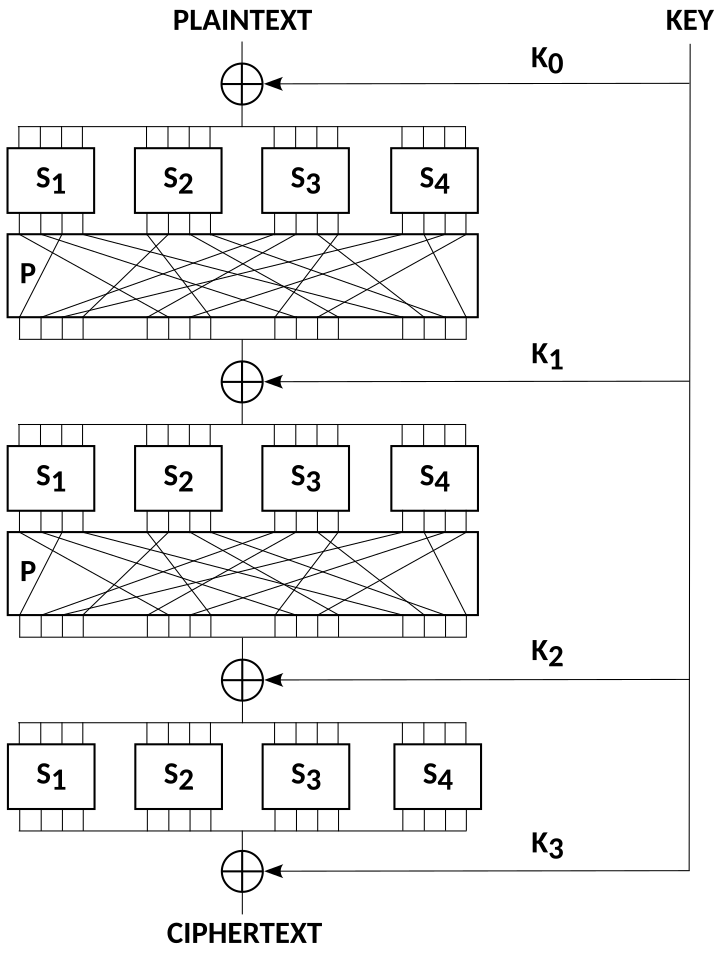
\includegraphics[width=\textwidth]{img/spn.png}
        \caption{A sketch of a substitution–permutation network with 3 rounds, encrypting a plaintext block of 16 bits into a ciphertext block of 16 bits. The S-boxes are the Si, the P-boxes are the same $P$, and the round keys are the $K_i$.}
        \label{fig:spn}
    \end{minipage}
    \hfill
    \begin{minipage}[t]{0.45\textwidth}
        \vspace{0pt} % Ensure top alignment
        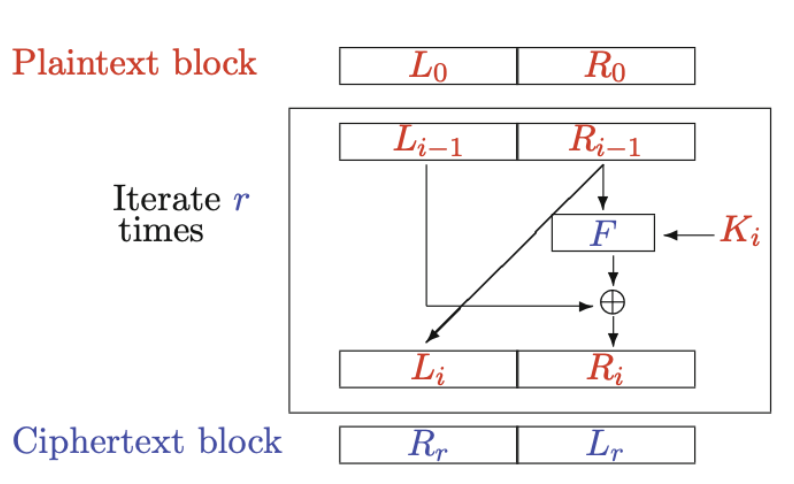
\includegraphics[width=\textwidth]{img/feistel.png}
        \caption{Basic operation of a Feistel cipher}
    \end{minipage}
\end{figure}

In a Feistel cipher, the round function is \emph{invertible}. It is different from an SPN, as that one is based on a non-invertible component. We can choose any function $F$ and still the round is invertible.
The same hardware/software can be used for encryption and decryption (just use the keys in reverse order). The security of the cipher depends on: the round keys, the number of rounds, and the function $F$.

\subsubsection{Encryption}
Given a plaintext block \( P \), a Feistel cipher processes it as follows:

\begin{enumerate}
    \item Initial split: Divide \( P \) into two equal-sized halves:
    \[
    P = (L_0, R_0)
    \]
    where \( L_0 \) and \( R_0 \) are the left and right halves, respectively.

    \item Rounds of encryption: For each round \( i \) (1 to \( n \)), compute:
    \[
    L_i = R_{i-1}
    \]
    \[
    R_i = L_{i-1} \oplus F(R_{i-1}, K_i)
    \]
    where:
    \begin{itemize}
        \item \( F \) is the round function (a non-linear function).
        \item \( K_i \) is the round key for round \( i \), derived from the main key.
    \end{itemize}

    \item Final Swap (Optional): After \( n \) rounds, the ciphertext \( C \) is obtained as:
    \[
    C = (R_n, L_n)
    \]
    (Note: The final swap is optional and does not affect decryption.)
\end{enumerate}

\subsubsection{Decryption}

The Feistel structure makes decryption straightforward because it is inherently reversible. Using the ciphertext \( C = (R_n, L_n) \):

\begin{enumerate}
    \item Initialize \( R_n \) and \( L_n \) as inputs.
    \item For each round \( i \) (in reverse order, from \( n \) to 1):
    \[
    R_{i-1} = L_i
    \]
    \[
    L_{i-1} = R_i \oplus F(L_i, K_i)
    \]
    \item Combine \( L_0 \) and \( R_0 \) to recover the original plaintext.
\end{enumerate}

The same function \( F \) and subkeys \( K_i \) are used in both encryption and decryption, but the subkeys are applied in reverse order during decryption.

\subsection{Data Encryption Standard (DES)}
DES is one of the earliest widely-used block ciphers. Not used anymore. But, still in ATMs (3DES). Key features are:

\begin{itemize}
    \item Block size: 64 bits
    \item Key length: 56 bits (with 8 parity bits)
    \item Number of rounds: 16
    \item 16 round keys, 48 bits each
    \item Structure: Feistel cipher
\end{itemize}

In the Feistel structure, each round splits the input into two halves: One half is directly passed to the next round. The other half is transformed using a combination of substitution, permutation, and the round key, then XORed with the other half.

\begin{figure}[h!]
    \centering
    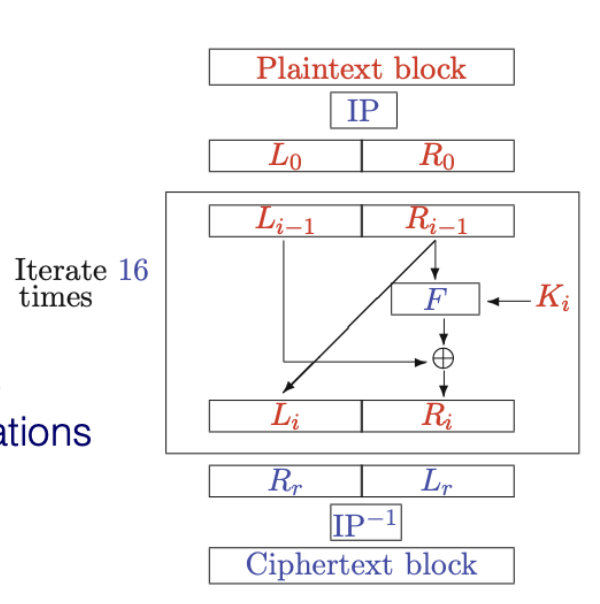
\includegraphics[width=0.35\textwidth]{img/des.png}
    \caption{DES as a Feistel structure}
    \label{fig:des}
\end{figure}

Operations:
\begin{itemize}
    \item 64 bits of plaintext block
    \item Perform an initial permutation (IP)
    \item Split the block into a left and right part
    \item Perform 16 rounds of \emph{identical operations}
    \item Join the half blocks together
    \item Perform a final reverse permutation (IP$^{-1}$)
\end{itemize}

\textbf{Decryption is identical to encryption: rounds keys in reversed order!} One algorithm is used for encryption and decryption. The same hardware can also be used for both.
DES is based on a Feistel structure. All that is needed to specify DES is a round function, a key schedule, and any additional processing (initial and final permutation).

\subsubsection{Function \texorpdfstring{$F$}{F}}
\begin{itemize}
    \item Expansion permutation: the right half 32 bits is expanded to 48 bits
    \item Round key addition: XOR with the round key 
    \item Splitting: 48 bits are split into 8 lots of 6-bit values
    \item S-boxes: non-linear part, output is 32 bits (8 lots of 4-bit values)
    \item P-box: Combine the previous lots to form a 32-bit value and apply permutation to form the output of $F$
\end{itemize}


\begin{figure}[h!]
    \centering
    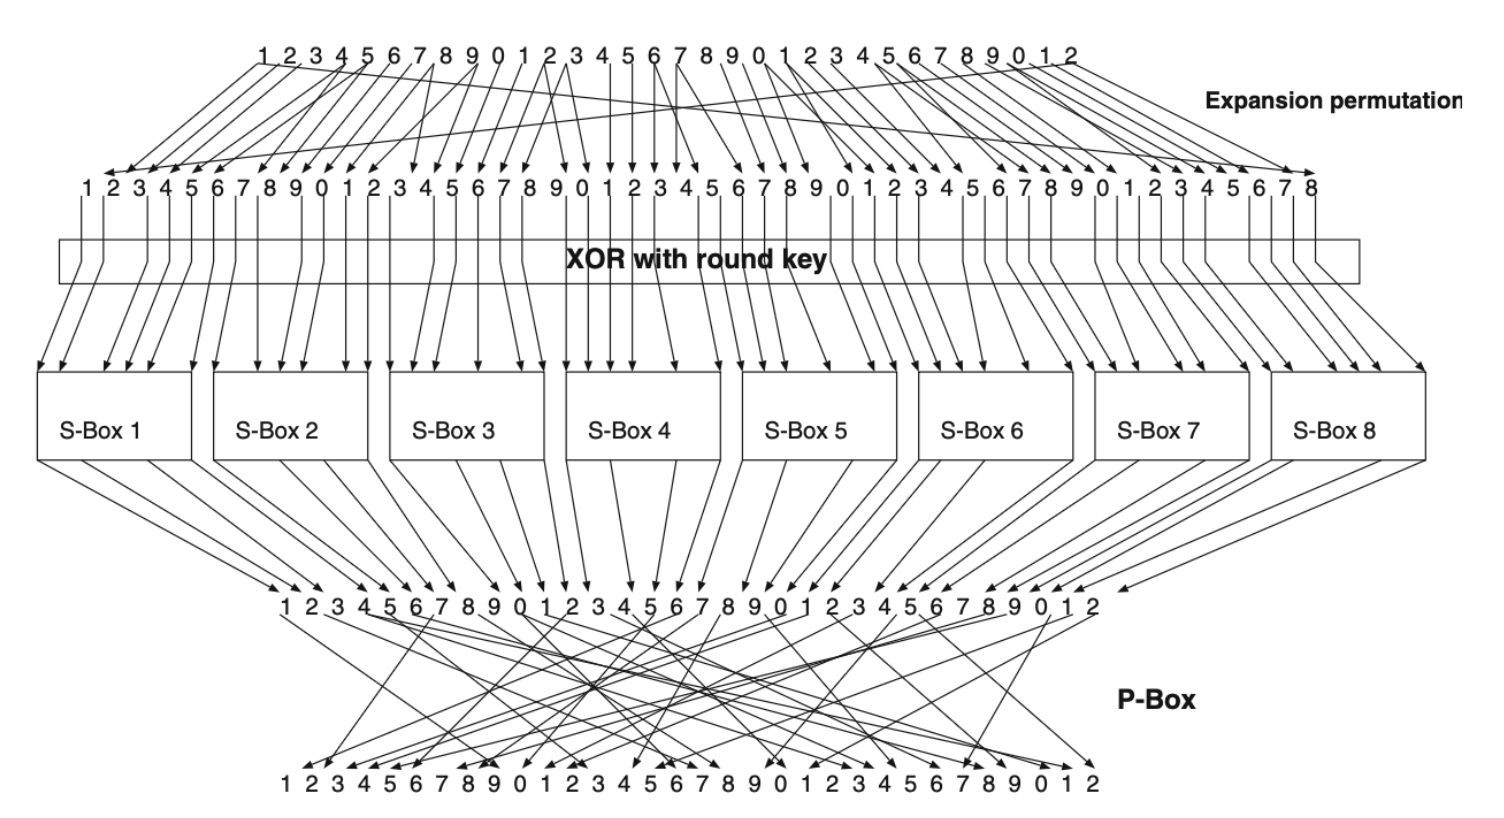
\includegraphics[width=0.5\textwidth]{img/desF.png}
    \caption{Structure of DES function \( F \)}
    \label{fig:f}
\end{figure}

\subsubsection{S-boxes}
In the \textbf{S-box} in the function $F$, the 48-bit result is divided into 8 groups of 6 bits. Each group of 6 bits is passed through a corresponding S-box, reducing it to 4 bits. \\

The S-box takes a 6-bit input and produces a 4-bit output. The 6-bit input is divided as follows:
\begin{itemize}
    \item The \textbf{first and last bits} (bits 1 and 6) are used to determine the \textbf{row number}.
    \item The \textbf{middle 4 bits} (bits 2, 3, 4, and 5) are used to determine the \textbf{column number}.
\end{itemize}

The row and column values are used to look up the corresponding 4-bit value in the S-box table (see lecture slides). DES uses 8 S-boxes, denoted \( S_1, S_2, \dots, S_8 \). Each S-box takes a 6-bit input and produces a 4-bit output. Together, the 8 S-boxes process the 48-bit input and reduce it to a 32-bit output.
The S-boxes are important for the following reasons:
\begin{itemize}
    \item Non-linearity: the S-box is the only non-linear component of the F-function, which makes DES resistant to linear and differential cryptanalysis.
    \item Confusion: S-boxes obscure the relationship between the plaintext, ciphertext, and the key.
    \item Compression: S-boxes reduce the 48-bit input to 32 bits, balancing the size for further processing.
\end{itemize}

\subsubsection{Permutations and P-box}
The \textbf{initial an final permutatations} are straight P-boxes that are inverses of each other. These permutations do not add cryptographic strength but are part of the standard DES algorithm.
\begin{itemize}
    \item The IP rearranges the 64-bit plaintext input bits into a new order. It is applied only once at the very beginning of the DES encryption process
    \item  The IP$^{-1}$ reverses the effect of the IP. It rearranges the bits of the 64-bit block back to their original positions
    \item IP and IP$^{-1}$ tables to specify how the input bits rearranged by index (see lecture slides for the tables)
\end{itemize}

The \textbf{expansion permutation} in the F-function of DES is a crucial step within each round of the encryption process. It is used to expand the 32-bit half-block input into 48 bits.
\begin{itemize}
    \item Bit duplication
    \item Introduce non-linearity: duplicating and rearranging bits makes it harder for an attacker to analyze relationships between plaintext, ciphertext, and the key.
    \item Kex mixing: XOR with the 48-bit round key
    \item Table in lecture slides
\end{itemize}

The \textbf{P-box} rearranges the bits of a given input in a specified order. The purpose of this permutation is to spread the influence of each bit across the output to enhance security by increasing diffusion. The P-box is used after the S-box substitution stage within the Feistel structure of DES. The S-box reduces the input to 32 bits, and the P-box permutes these 32 bits to prepare them for the next round of processing.

\subsubsection{Key Scheduling}
The \textbf{Key scheduling} process in DES generates 16 \textbf{subkeys} (48 bits each) from the original \textbf{64-bit key}. These subkeys are used in the 16 Feistel rounds of DES encryption. The key scheduling process consists of the following main steps:
\begin{enumerate}
    \item Initial 64-bit key is reduced to 56 bits by removing parity bits using the \textbf{PC-1} table.
    \item The 56-bit key is split into two 28-bit halves: \( C_0 \) and \( D_0 \).
    \item For each of the 16 rounds, both halves undergo \textbf{left circular shifts} (1 or 2 bits depending on the round).
            \[ C_i \leftarrow C_{i-1} \lll p_i \]
            \[ D_i \leftarrow D_{i-1} \lll p_i \]

        where $p_i$ is the cyclic shift.
    \item Combine the two halves. The \textbf{PC-2} table compresses the 56-bit key (combined \( C_i \) and \( D_i \)) into a 48-bit subkey.
    \item This process is repeated 16 times to generate 16 unique subkeys.
\end{enumerate}

\begin{figure}[h!]
    \centering
    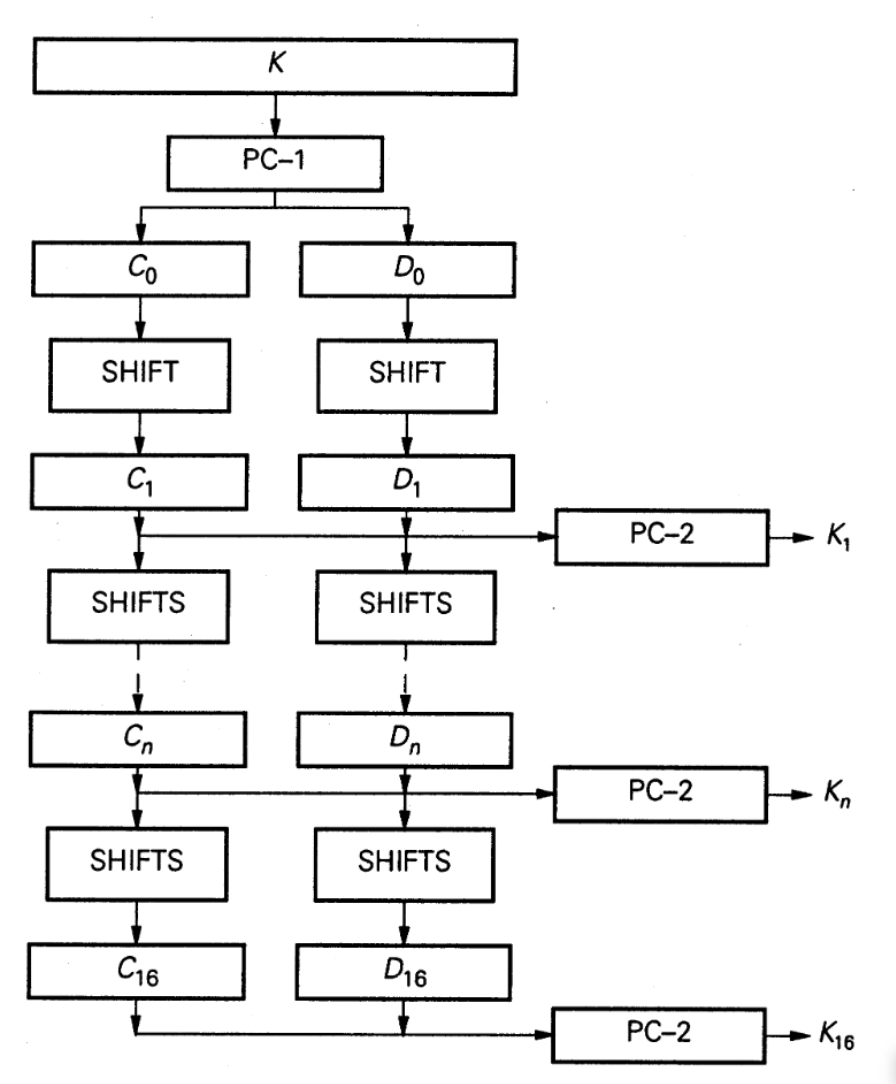
\includegraphics[width=0.3\textwidth]{img/DESkey.png}
    \caption{DES key scheduling}
    \label{fig:key}
\end{figure}

The key schedule ensures that even a small change in the original key produces completely different subkeys.




\subsubsection{Security of DES}
1, 2, and 3-round DES is not secure. DES in general is not secure! Can be cracked with exhaustive search. But: costs a lot of time or memory. Time-space tradeoff: with more memory, a few minutes is sufficient. The 56-bit key length is vulnerable to brute-force attacks (exhaustive search). Modern computational power can crack DES in hours. 
However, to crack DES you need mathematical, puzzle-solving skills and \emph{luck}. \\

The key length is the weakest point in DES. Then can't we just encrypt twice, using two keys? The key space would become $2^{n\cdot k} = 2^{112}$ with $n = 2, k = 56$. Unfortunately, this is not true. The key space remains $2^{56}$:

When trying to improve the security of a block cipher, a tempting idea is to encrypt the data several times using multiple keys. One might think this doubles or even n-tuples the security of the multiple-encryption scheme, depending on the number of times the data is encrypted, because an exhaustive search on all possible combinations of keys (simple brute force) would take $2^{n\cdot k}$ attempts if the data is encrypted with $k$-bit keys $n$ times. \\

\begin{figure}[h!]
\centering
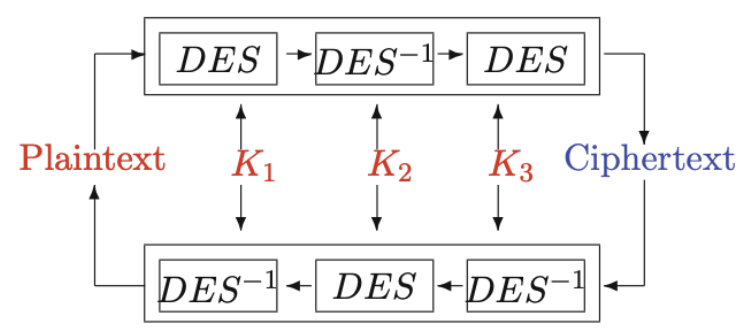
\includegraphics[width=0.4\textwidth]{img/3DES.png}
\caption{Triple DES}
\end{figure}

The \textbf{meet-in-the-middle attack} (MITM) is a generic attack that weakens the security benefits of using multiple encryptions by storing intermediate values from the encryptions or decryptions and using those to improve the time required to brute force the decryption keys. 
The attack attempts to find the keys by using both the range (ciphertext) and domain (plaintext) of the composition of several functions (or block ciphers) such that the forward mapping through the first functions is the same as the backward mapping (inverse image) through the last functions, quite literally meeting in the middle of the composed function. For example, although Double DES encrypts the data with two different 56-bit keys, Double DES can be broken with $2^{57}$ encryption and decryption operations.
The MITM attack is the primary reason why 2DES is not used, and 3DES can be brute-forced by an attacker with $2^{56}$ space and $2^{112}$ operations.


\subsubsection{Cryptanalysis of Block Ciphers}
Can be done with:
\begin{itemize}
    \item Exhaustive search
    \item Pre-computed intermediate values
    \item Divide and conquer
\end{itemize}

A block cipher should be resistant against differential and linear cryptanalysis. \Comment{explain what this is?}

\subsection{Advanced Encryption Standard (AES)}
AES replaced DES in the 1990s. Public design. AES is not a Feistel cipher, but a SPN. It is based on the Rijndael algorithm. Key features are:
\begin{itemize}
    \item Each round has a key addition phase, a substitution phase (non-linear, confusion), and a permutation phase (for diffusion, avalanche effect)
    \item AES is built on a mathematical foundation (finite fields $\mathbb{F}_{2^8}, \mathbb{F}_2$)
    \item Encryption and decryption are distinct operations (do not rely \emph{solely} on reverse ordering of the keys)
    \item Supports multiple key lengths: 128, 192, and 256 bits (and thus also blocks of these sizes)
\end{itemize}

\subsubsection{Finite Fields and Arithmatic in AES}
Elements of $\mathbb{F}_{2^8}$ are stored as bit vectors (or bytes) representing \textbf{binary polynomials}. From the hexadecimal representation of a byte, we can derive the polynomial representation. For example, the byte \texttt{0x57} is represented by the polynomial $x^6 + x^4 + x^2 + x + 1$. The polynomial representation is used for arithmetic operations in AES.

\[ \texttt{0x57} = 5 \cdot 16 + 7 = 87 \] in decimal. The bit representation in binary is given by concatenating the bit representation of 5 and 7:

\[\texttt{0101 0111}\]

The bit pattern then corresponds to the binary polynomial, using the indexes where the bits are set to 1 as the exponents of the polynomial:

\[ x^6 + x^4 + x^2 + x + 1\] 

Arithmethic in the finite field $\mathbb{F}_{2^8}$ is a cornerstone of the AES algorithm. It is a Galois field with $2^8 = 256$ elements. \\

\textbf{Field Construction}
\begin{itemize}
    \item \(\mathbb{F}_{2^8}\) is constructed as a polynomial field over \(\mathbb{F}_2\) (the field with two elements, \(0\) and \(1\)).
    \item Elements of \(\mathbb{F}_{2^8}\) are represented as polynomials of degree at most 7 with coefficients in \(\mathbb{F}_2\). For example:
    \[
    a(x) = a_7x^7 + a_6x^6 + \cdots + a_1x + a_0, \quad a_i \in \{0, 1\}.
    \]
    \item Addition and multiplication of elements are defined modulo an irreducible polynomial \(m(x)\) of degree 8 over \(\mathbb{F}_2\). In AES, the chosen irreducible polynomial is:
    \[
    m(x) = x^8 + x^4 + x^3 + x + 1.
    \]
\end{itemize}

\textbf{Addition}
\begin{itemize}
    \item Addition in \(\mathbb{F}_{2^8}\) corresponds to bitwise XOR of the coefficients of the two polynomials.
    \item Example:
    \[
    (a_7x^7 + a_6x^6 + \cdots + a_0) + (b_7x^7 + b_6x^6 + \cdots + b_0)
    = (a_7 \oplus b_7)x^7 + \cdots + (a_0 \oplus b_0).
    \]
\end{itemize}

\textbf{Multiplication}
\begin{enumerate}
    \item \textbf{Polynomial Multiplication}:
    \begin{itemize}
        \item Multiply two polynomials \(a(x)\) and \(b(x)\) normally, treating them as polynomials over \(\mathbb{F}_2\).
        \item Example:
        \[
        a(x) = x^2 + 1, \quad b(x) = x^3 + x
        \]
        \[
        a(x) \cdot b(x) = (x^2 + 1)(x^3 + x) = x^5 + x^3 + x^3 + x = x^5 + x.
        \]
    \end{itemize}
    \item \textbf{Modulo Reduction}:
    \begin{itemize}
        \item Reduce the result modulo the irreducible polynomial \(m(x)\).
        \item For example, if \(a(x) \cdot b(x) = x^9 + x^5\), reduce it modulo \(x^8 + x^4 + x^3 + x + 1\):
        \[
        x^9 = x \cdot x^8 \equiv x(x^4 + x^3 + x + 1) \mod m(x).
        \]
    \end{itemize}
    \item The final result after reduction is the product in \(\mathbb{F}_{2^8}\).
\end{enumerate}

\textbf{Inversion}
\begin{itemize}
    \item Inversion (finding the multiplicative inverse) is critical in the AES S-box.
    \item The inverse of an element \(a(x)\) in \(\mathbb{F}_{2^8}\) is the unique element \(b(x)\) such that:
    \[
    a(x) \cdot b(x) \equiv 1 \mod m(x).
    \]
    \item This is typically computed using the Extended Euclidean Algorithm.
\end{itemize}

\subsubsection{State Matrix}
AES organizes the input plaintext (or ciphertext) as a 4x4 matrix of bytes called the state. Each entry in the matrix is one byte (8 bits), and the matrix evolves through each round of AES encryption or decryption. Each round key is held by a 4x4 matrix.

\[ S = \begin{pmatrix}
    s_{0,0} & s_{0,1} & s_{0,2} & s_{0,3} \\
    s_{1,0} & s_{1,1} & s_{1,2} & s_{1,3} \\
    s_{2,0} & s_{2,1} & s_{2,2} & s_{2,3} \\
    s_{3,0} & s_{3,1} & s_{3,2} & s_{3,3} \\
\end{pmatrix},
K_i = \begin{pmatrix}
    k_{0,0} & k_{0,1} & k_{0,2} & k_{0,3} \\
    k_{1,0} & k_{1,1} & k_{1,2} & k_{1,3} \\
    k_{2,0} & k_{2,1} & k_{2,2} & k_{2,3} \\
    k_{3,0} & k_{3,1} & k_{3,2} & k_{3,3} \\
\end{pmatrix} \] \\

\textbf{Mapping Input Plaintext to the State Matrix}
\begin{itemize}
    \item AES operates on 128-bit blocks (16 bytes) at a time.
    \item The 128-bit plaintext block is split into 16 bytes and arranged column-by-column into the state matrix.
\end{itemize}

For a plaintext block:
\[
P = [\text{byte}_0, \text{byte}_1, \dots, \text{byte}_{15}],
\]
the state matrix is represented as:
\[
S = 
\begin{pmatrix}
\text{byte}_0 & \text{byte}_4 & \text{byte}_8  & \text{byte}_{12} \\
\text{byte}_1 & \text{byte}_5 & \text{byte}_9  & \text{byte}_{13} \\
\text{byte}_2 & \text{byte}_6 & \text{byte}_{10} & \text{byte}_{14} \\
\text{byte}_3 & \text{byte}_7 & \text{byte}_{11} & \text{byte}_{15}
\end{pmatrix}.
\]

\subsubsection{AES Operations}
The state array is manipulated using four main operations: SubBytes, ShiftRows, MixColumns, and AddRoundKey. These operations are repeated for multiple rounds, with the number of rounds depending on the key length. \\

\begin{figure}[h!]
    \centering
    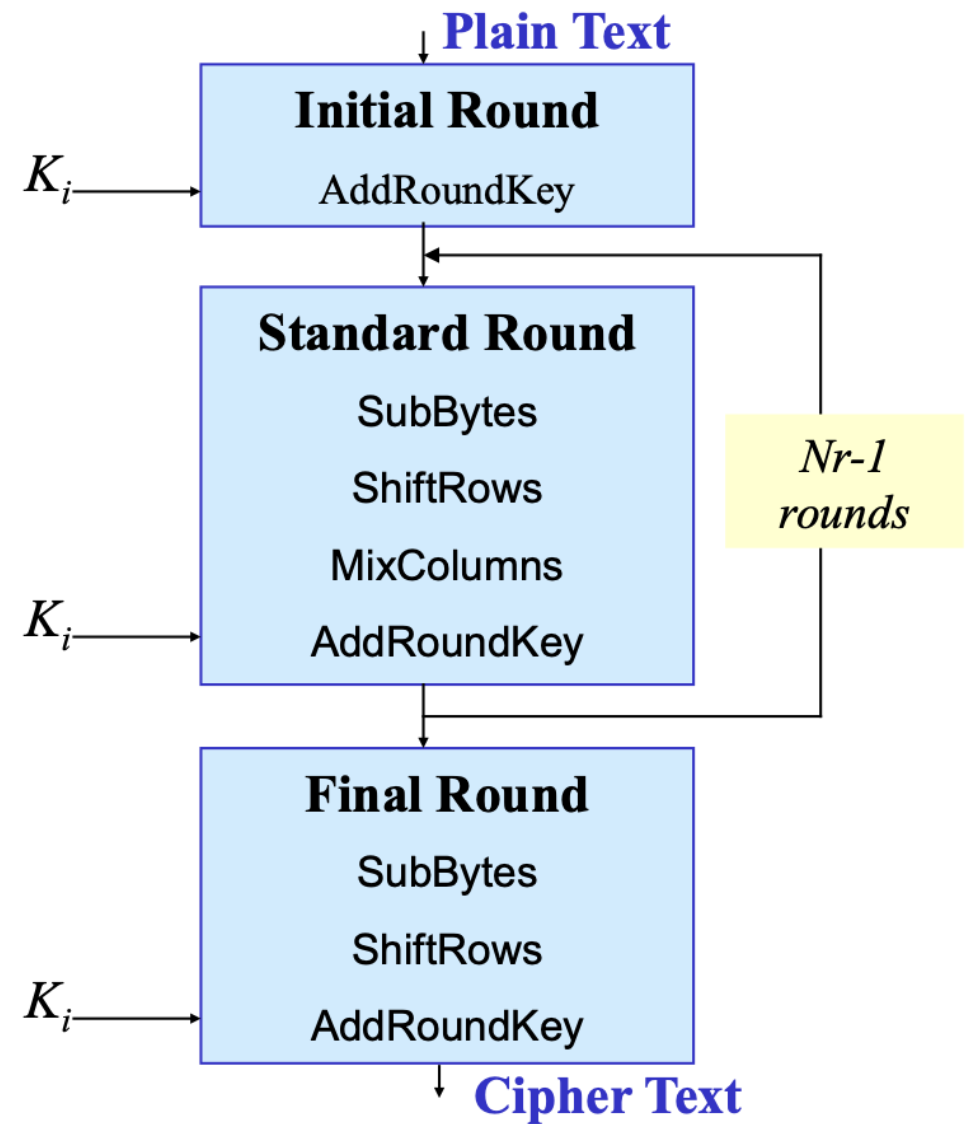
\includegraphics[width=0.3\textwidth]{img/AES.png}
    \caption{Overview of rounds in AES encryption}
    \label{fig:aes}
\end{figure}

\textbf{AddRoundKey}
This operatation takes the state matrix and XORs it, byte by byte, with the round key matrix. The inverse of this operation is clearly the same operation. \\

\textbf{SubBytes}\\
The SubBytes operation in the AES algorithm is a simple substitution step that replaces each byte in the state with another byte using a fixed substitution box (S-box).
Criteria for S-Box:
\begin{itemize}
    \item S-box must be resistant against linear and differential cryptanalysis
    \item S-box must be simple
    \item S-box must be invertible
\end{itemize}

\textbf{ShiftRows}
The ShiftRows operation performs a cyclic shit on the state matrix. Each row is shifted by a different offset (row 1 with 0, row 2 with 1, etc.) \\

\textbf{MixColumns}
This operation ensures that the rows in the state matrix ``interact" with each other over a number of rounds; combined with the ShiftRows operation it ensures each byte of the output state depends on each byte of the input state.
Each column in the state $[ a_0, a_1, a_2, a_3]$ is considered one at a time to create a new column $[b_0, b_1, b_2, b_3]$. This is done by taking the polynomial
\[ a(X) = a_0 + a_1 \cdot X + a_2 \cdot X^2 + a_3 \cdot X^3 \]
and multiplying it by the polynomial $c(X)$ that was chosen for AES to maximize diffusion.
\[ 
c(X) = \texttt{0x02} + \texttt{0x01} \cdot X + \texttt{0x01}  \cdot X^2 + \texttt{0x03}  \cdot X^3
\]

Then the modulo is taken with the invertible polynomial $M(X)$ to ensure invertibility of the MixColumns operation.

\[ M(X) = X^4 + 1 \]

This can be represented by a multiplication matrix (see book and slides) that is invertible in $\mathbb{F}_{2^8}$.


\begin{figure}[h!]
    \centering
    \begin{subfigure}[t]{0.45\textwidth}
        \centering
        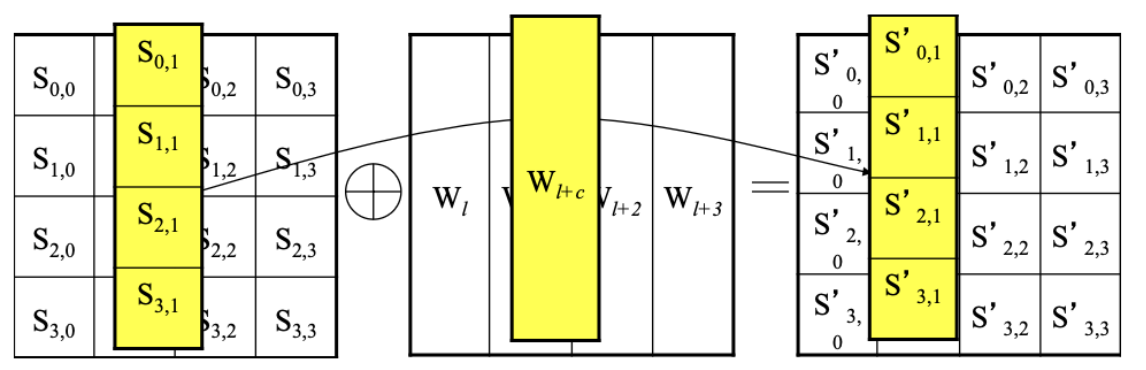
\includegraphics[width=\textwidth]{img/addroundkey.png}
        \caption{Add Round Key}
    \end{subfigure}
    \hfill
    \begin{subfigure}[t]{0.45\textwidth}
        \centering
        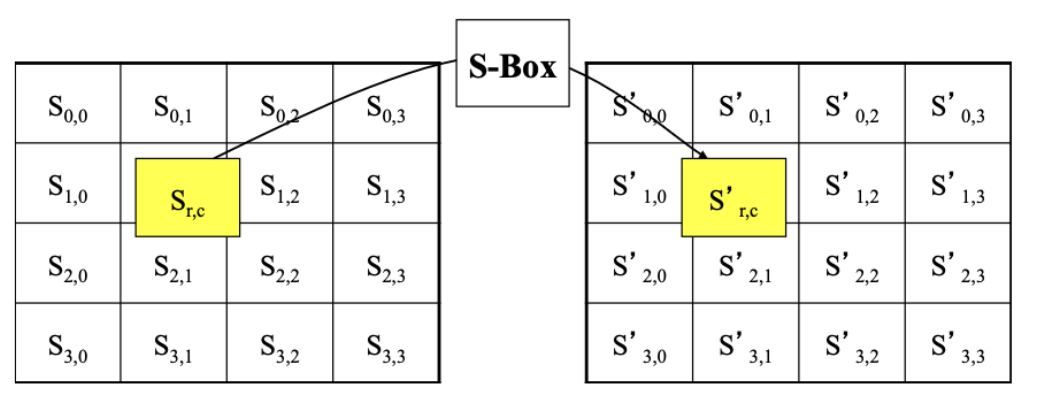
\includegraphics[width=\textwidth]{img/subbytes.png}
        \caption{Sub Bytes}
    \end{subfigure}
    \vfill
    \begin{subfigure}[t]{0.45\textwidth}
        \centering
        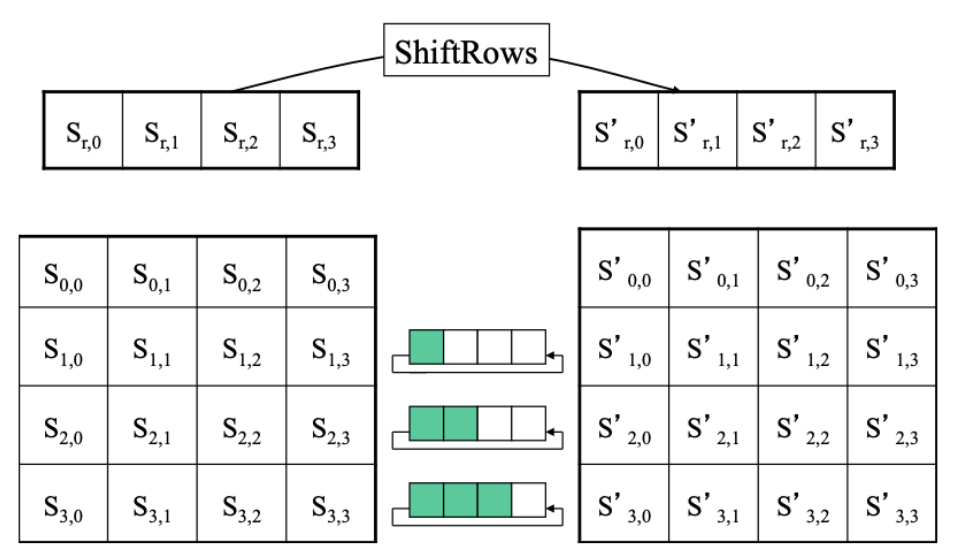
\includegraphics[width=\textwidth]{img/shiftrows.png}
        \caption{Shift Rows}
    \end{subfigure}
    \hfill
    \begin{subfigure}[t]{0.45\textwidth}
        \centering
        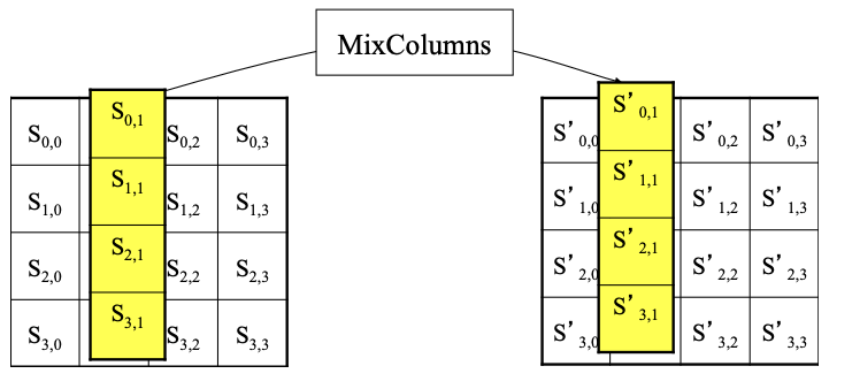
\includegraphics[width=\textwidth]{img/mixcolumns.png}
        \caption{Mix Columns}
    \end{subfigure}
    \caption{AES Operations visualized}
    \label{fig:aes-operations}
\end{figure}

\subsubsection{Key Scheduling}
The AES key schedule generates a series of round keys from the initial secret key. These round keys are used in each round of AES encryption or decryption. Here, we focus on AES with 128-bit blocks. \\


The main key is 128 bits long, and we need to produce 11 round keys $K_0,...,K_{11}$ all of which consist of four 32-bit words, each word corresponding to a column of the matrix K as described above.
The secret key is split into 4-byte words: for AES-128, the key has 4 words \( W_0, W_1, W_2, W_3 \). 
AES requires a separate \textbf{round key} for each encryption round, here: 10 rounds → 11 round keys (each 16 bytes). The round keys are derived using a process called \textbf{key expansion}:

\begin{itemize}
    \item \textbf{RotWord}:
    \begin{itemize}
        \item Rotate the bytes in a word to the left by one position.
        \item Example: \( [b_0, b_1, b_2, b_3] \rightarrow [b_1, b_2, b_3, b_0] \).
    \end{itemize}
    
    \item \textbf{SubWord}:
    \begin{itemize}
        \item Substitute each byte of the word using the AES S-box (just like in the SubBytes step of AES).
    \end{itemize}
    
    \item \textbf{RC}:
    \begin{itemize}
        \item Add a constant value, called the \textbf{round constant}, to the first byte of the word. This ensures that each round key is different.
    \end{itemize}
\end{itemize}

\Comment{Finish this later, i dont really get it...}

\begin{figure}[h!]
    \centering
    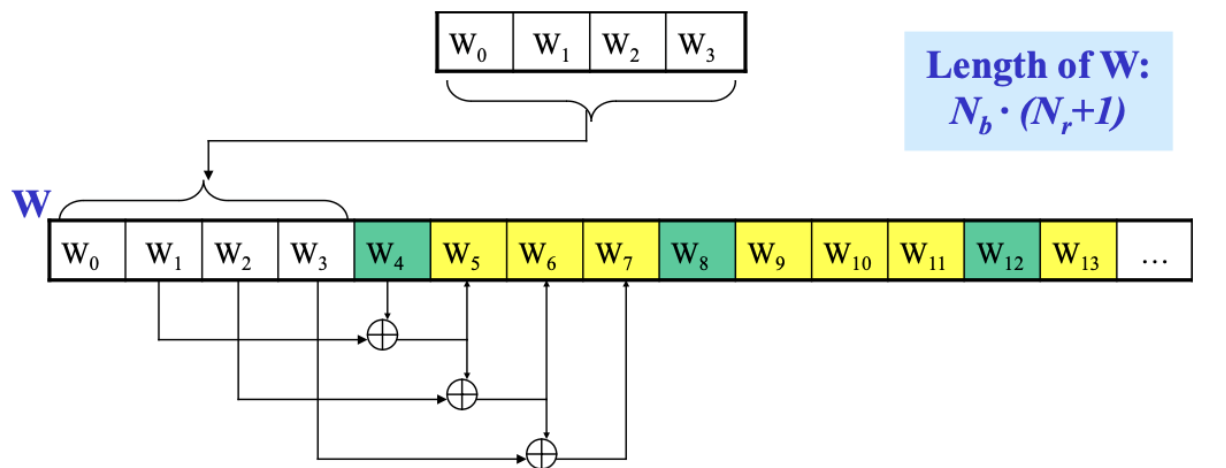
\includegraphics[width=0.5\textwidth]{img/AESkeyschedule.png}
    \caption{AES Key Scheduling}
\end{figure}

\subsubsection{Encryption and Decryption}

\begin{figure}[h!]
    \centering
    \begin{subfigure}[t]{0.40\textwidth}
        \centering
        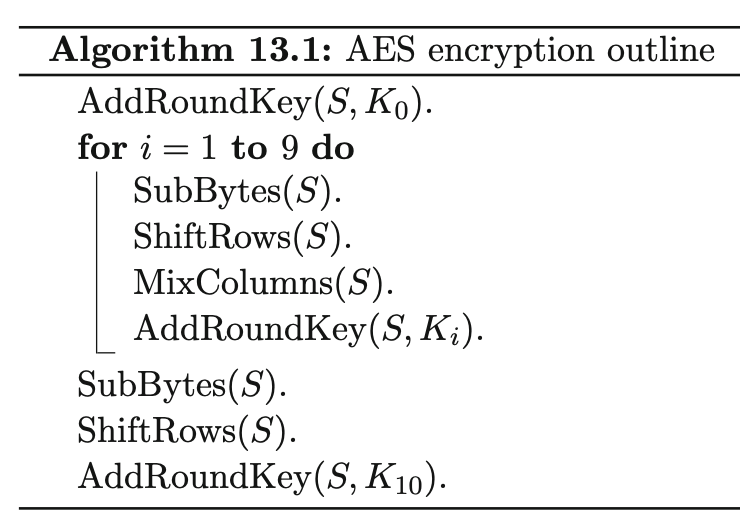
\includegraphics[width=\textwidth]{img/AESencrypt.png}
        \end{subfigure}
        \hfill
        \begin{subfigure}[t]{0.40\textwidth}
            \centering
            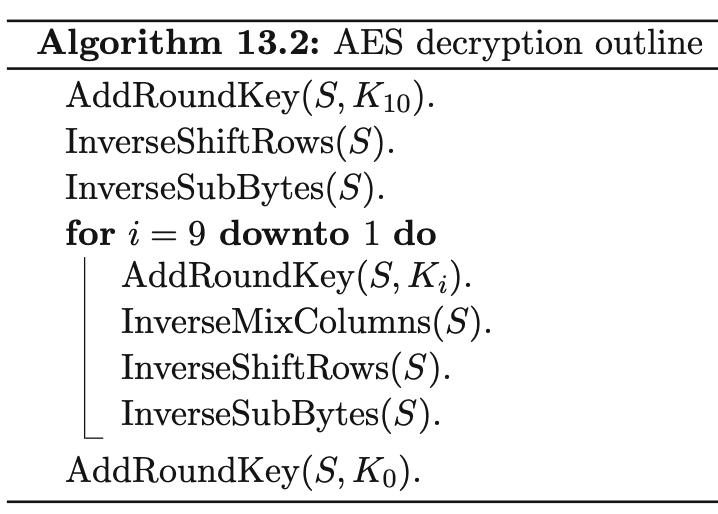
\includegraphics[width=\textwidth]{img/AESdecrypt.png}
        \end{subfigure}
    \caption{Pseudocode for AES Encryption and Decryption}
\end{figure}

\subsection{DES vs. AES}
\begin{table}[h!]
    \centering
    \begin{tabular}{|>{\raggedright\arraybackslash}m{4cm}|>{\raggedright\arraybackslash}m{6cm}|>{\raggedright\arraybackslash}m{6cm}|}
    \hline
    \textbf{Feature} & \textbf{DES} & \textbf{AES} \\
    \hline
    Performance & Fast in hardware, slower in software & Fast in hardware and software \\
    \hline
    Key Length & One key length (not expandable) & Multiple key lengths (expandable in the future) \\
    \hline
    Block Length & One block length (not expandable) & Multiple block lengths \\
    \hline
    Number of Iterations & Many iterations (Feistel structure) & Relatively small amount of iterations \\
    \hline
    \end{tabular}
    \caption{Comparison of DES and AES}
\end{table}



\subsection{Modes of Operation}
Originally, 4 standard modes:
\begin{itemize}
    \item ECB (Electronic Codebook)
    \item CBC (Cipher Block Chaining)
    \item CFB (Cipher Feedback)
    \item OFB (Output Feedback)
\end{itemize}

Over the years, many more: CTR (Counter Mode)

\subsubsection{Electronic Codebook (ECB)}

\subsubsection{Cipher Block Chaining (CBC)}

\subsubsection{Cipher Feedback (CFB)}

\subsubsection{Output Feedback (OFB)}

\subsubsection{Counter Mode (CTR)}

\subsubsection{Security: how to achieve CCA?}

\newpage

\section{Lecture 8}

\subsection{Hash Functions}

\subsection{Collision Resistance}

\subsection{Padding}

\subsection{Merkle-Damg\aa rd Construction}

\subsection{Birthday Paradox}

\subsection{MD-family}

\subsection{MAC}

\subsection{Sponge Functions}

\newpage 
\section{Lecture 9}

Symmetric encryption algorithms are fast and efficient because they use a single shared key for both encryption and decryption.
However, the \textbf{key distribution problem} arises because both parties must securely share the secret key before any communication can occur. 
Secure transmission of the key, no built-in key exchange mechanism in the encryption scheme, scalability in systems with multiple uses (number of unique keys grows exponentially), risk of compromise, etc. \\

Solution: use \textbf{public-key cryptography} (asymmetric encryption) to securely exchange keys.
Public key encryption algorithms are slow, but key distribution is easier.
Public key is broadcasted, private key is kept secret.

\subsection{Naive RSA Algorithm}
Based on the difficulty of factoring large numbers that are the product of two (large) prime numbers.
Multiplying these two numbers is easy, but determining the original prime numbers from the total -- or factoring -- is considered infeasible due to the time it would take using even today's supercomputers. \\

Given a large composite number $N$, find $d$ given $e$. It works as follows:
\begin{enumerate}
\item Alice chooses two large primes $p$ and $q$
\item Alice computes $N = pq$
\item Alice chooses $e$ such that $\gcd(e, (p-1)(q-1)) = 1$, i.e., $e$ is relatively prime to $(p-1)(q-1)$, which is the totient function of $N$
\item Alice computes $d$ such that $ed \equiv 1 \pmod{(p-1)(q-1)}$, i.e., $d$ is the modular multiplicative inverse of $e$ modulo $\phi(N)$
\end{enumerate}

The public key is $(N, e)$ and the private key is $(N, d)$, $(p, q, d)$, $(p,q)$, or $(d)$. \Comment{why do all these work?}

\subsubsection{Encryption and Decryption}
To encrypt a message $m$ (converted to a numeric value), compute:
\[ C = m^e \mod N \]

where C is the ciphertext. To decrypt the ciphertext, compute:

\[ m = C^d \mod N \]

The RSA algorithm works due to the following:
\[
x^{(p-1)(q-1)} \equiv 1 \pmod{N}, \quad \text{for all } x \in \mathbb{Z}/N\mathbb{Z}^*,
\]
where \( \mathbb{Z}/N\mathbb{Z}^* \) is the set of integers coprime to \( N \). This ensures that certain powers of \( x \) ``wrap around" in modular arithmetic (Euler's theorem).
The public key exponent \( e \) and the private key exponent \( d \) are chosen such that:
\[
e \cdot d \equiv 1 \pmod{\phi(N)}.
\]
This implies:
\[
e \cdot d - s \cdot \phi(N) = 1,
\]
where \( s \) is an integer. Thus, \( d \) is the modular multiplicative inverse of \( e \) modulo \( \phi(N) \).
Substituting \( c = m^e \) in the decryption equation, we get:
\[
m = (m^e)^d \pmod{N}.
\]
Since \( e \cdot d = 1 + s \cdot \phi(N) \), we can rewrite this as:
\[
m^{ed} = m^{1 + s \cdot \phi(N)} = m^1 \cdot (m^{\phi(N)})^s.
\]
By Euler's theorem, \( m^{\phi(N)} \equiv 1 \pmod{N} \), so:
\[
m \cdot 1^s = m \pmod{N}.
\]

\subsubsection{Example of RSA}

Let\( p = 47 \), \( q = 59 \), and \( N = p \cdot q = 2773 \). Then \( \phi(N) = (p-1)(q-1) = 2668 \). We pick \( e = 17 \).
Now, find \( d \) such that \( e \cdot d \equiv 1 \pmod{\phi(N)} \): 
    \[
    17 \cdot d \equiv 1 \pmod{2668}, \quad \text{so } d = 157.
    \]

 Plaintext Message (\( M \)): \texttt{ITS ALL GREEK TO ME}. Convert to numeric format:
    \[
    M = 0920 \, 1900 \, 0112 \, 1200 \, 0718 \, 0505 \, 1100 \, 2015 \, 0013 \, 0500.
    \]

Ciphertext (\( C \)) is calculated as:
    \[
    C = M^e \pmod{N}.
    \]
Result:
    \[
    C = 0948 \, 2342 \, 1084 \, 1444 \, 2663 \, 2390 \, 0778 \, 0774 \, 0219 \, 1655.
    \]
Encrypt a portion: 
    \[
    920^{17} \pmod{2773}.
    \]
    
Decrypt a portion:
    \[
    948^{157} \pmod{2773}.
    \]


\begin{figure}[h!]
    \centering
    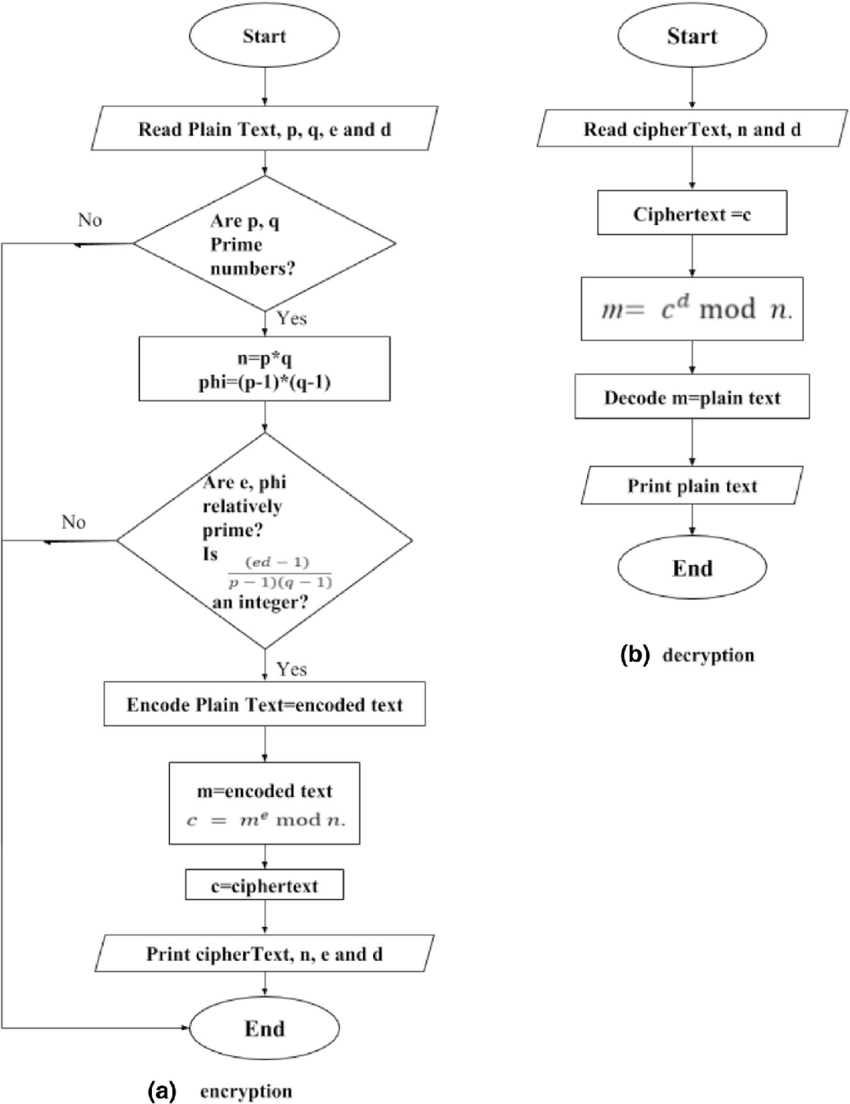
\includegraphics[width=0.5\textwidth]{img/Block-diagram-of-RSA-algorithm.png}
    \caption{RSA Algorithm}
\end{figure}

\subsection{Security of RSA}
Computing $d$ given $e$ and $N$ is equivalent to factoring $N$ into its prime factors $p$ and $q$. Thus it is no harder than factoring $N$. 
Current suggestion: modulo need to be 2048 bits long. RSA is OW-CPA, but not IND-CPA secure, because:
\begin{itemize}
    \item Deterministic encryption: same plaintext always encrypts to the same ciphertext
    \item No randomness
    \item Mathematical structure leaks information: 
        \[ (M_1 \cdot M_2)^e = M_1^e \cdot M_2^e \]
        Atttacker can gain information about plaintexts from ciphertext relationships
    \item Chosen plaintext attacks: attacker can guess relationshup between plain- and cipher text due to deterministic nature and lack of padding
\end{itemize}

But, deterministic encryption is not the only problem: RSA is \textbf{malleable} due to homomorphism.

\begin{defn}
\textbf{Homomorphic Property:} an encryption scheme has the (multiplicate) homomorphic property if given the encryptions of $m_1$ and $m_2$
we can determine the encryption of $m_1 \cdot m_2$ without knowing $m_1$ or $m_2$.
\end{defn}

RSA is multiplicatively homomorphic:

\[ (m_1 \cdot m_2)^e = ((m_1^e \pmod{N}) \cdot (m_2^e \pmod{N})) \pmod{N} \]

The naive RSA is \emph{not} OW-CCA secure. Remember that we hae a decryption oracle:

\[ c^* = (m^*)^e \pmod{N} \]
\[ c = 2^e \cdot c^* \]
\[ \frac{m}{2} = \frac{c^d}{2} = \frac{(2^e \cdot c^*)^d}{2} \]

\[ = \frac{2^{ed} \cdot (c^*)^d}{2} = \frac{2 \cdot m^*}{2} = m^*\]


\subsubsection{How to make RSA IND-CPA secure?}

To achieve \textbf{IND-CPA} security, RSA requires modifications, such as the use of \textbf{randomized padding schemes}. Below are two common approaches:

\begin{enumerate}
    \item RSA-OAEP (Optimal Asymmetric Encryption Padding)
\begin{itemize}
    \item OAEP introduces \textbf{randomness} to the plaintext before applying the RSA encryption formula.
    \item This randomness ensures that even if the same plaintext is encrypted multiple times, the resulting ciphertexts will differ.
    \item RSA with OAEP is considered \textbf{IND-CPA secure in practice}.
\end{itemize}

\item Hybrid Encryption
\begin{itemize}
    \item RSA is often combined with \textbf{symmetric encryption} in real-world protocols.
    \item RSA is used to encrypt a randomly generated \textbf{symmetric key}, ensuring IND-CPA security for the key exchange.
    \item The symmetric key is then used to encrypt the actual message, leveraging the efficiency of symmetric encryption.
\end{itemize}
\end{enumerate}

\subsection{Rabin Encryption}
Public key encryption scheme based on integer factoriziation. It is similar to RSA, but the encryption and decryption functions are different. 
Rabin encryption is based on a \textbf{trapdoor function}, having the advantage that inverting it is as hard as factoring intergers. RSA however, lacks this equivalence. \\
OW-CPA secure based in factoring problem. Mapping is not injective. \Comment{what does that mean?}

\subsubsection{Key Generation}
Choose two large prime numbers \( p \) and \( q \), such that \( p \equiv 3 \pmod{4} \) and \( q \equiv 3 \pmod{4} \).
Compute \( N = p \cdot q \), where \( N \) is the public modulus.
The \textbf{public key} is \( N \), and the \textbf{private key} is \( (p, q) \).
So, everyone can encrypt a message using \( N \), but only the owner of \( p \) and \( q \) can decrypt it. There is no need of $N$ at the receiver side.

\subsubsection{Encryption and Decryption}
To encrypt a message \( M \) (converted to a numeric value \( M \) such that \( 0 \leq M < N \)):
    \[
    C = M^2 \pmod{N}.
    \]
\( C \) is the ciphertext. \\

Given the ciphertext \( C \), the decryption process involves finding the \textbf{square roots} of \( C \) modulo \( N \).
Using the Chinese Remainder Theorem (CRT), the decryption yields \textbf{four possible solutions}:
   
\[ m_p = \sqrt{c} \pmod{p} = c^{(p+1)/4} \pmod{p}\]

\[ m_q = \sqrt{c} \pmod{1} = c^{(1+1)/4} \pmod{1}\]

\[
    m_1, m_2, m_3, m_4.
    \]
The correct plaintext \( m \) out of the 4 possible ones must be determined using additional information or context.

\subsubsection{Trapdoor}
The trapdoor here is the ability to efficiently compute square roots $N = p\cdot q$ when you know the two prime factors. You can use the CRT to compute the sqaure roots efficiently. \\

To encrypt, the sender computes the ciphertext \( C \) as:
\[
C = M^2 \pmod{N}.
\]
Given only \( N \), recovering \( M \) from \( C \) requires computing the square root of \( C \pmod{N} \), which is difficult unless the factors \( p \) and \( q \) are known.

When the receiver knows the private key (the factors \( p \) and \( q \)):
\begin{itemize}
    \item The receiver solves two modular equations:
    \[
    M^2 \equiv C \pmod{p}, \quad M^2 \equiv C \pmod{q}.
    \]
    Since \( p \) and \( q \) are primes, these equations can be solved efficiently using modular arithmetic techniques (such as modular square root algorithms).

    \item Using the CRT, the receiver combines the solutions modulo \( p \) and \( q \) to compute four possible square roots modulo \( N \).
\end{itemize}

The decryption produces \textbf{four possible square roots} because:
\begin{itemize}
    \item For a given \( p \), there are two solutions: \( M \pmod{p} \) and \( -M \pmod{p} \).
    \item Similarly, for \( q \), there are two solutions: \( M \pmod{q} \) and \( -M \pmod{q} \).
\end{itemize}
Using the CRT, these combine to produce four distinct solutions modulo \( N \). The receiver must use additional context (e.g., padding) to identify the correct plaintext.

\begin{itemize}
    \item Without knowing \( p \) and \( q \), the decryption problem is as hard as factoring \( N \). Factoring large composite numbers is computationally infeasible with current algorithms for sufficiently large \( N \), making this a secure one-way function.
    \item Knowing \( p \) and \( q \) provides a "backdoor" (the trapdoor) to efficiently decrypt the ciphertext by finding square roots modulo \( N \).
\end{itemize}

\textbf{Analogy with RSA}
\begin{itemize}
    \item In RSA, the trapdoor is the knowledge of \( \phi(N) = (p-1)(q-1) \) (or equivalently \( p \) and \( q \)), which allows the computation of the private key \( d \), the modular inverse of the public key \( e \) modulo \( \phi(N) \).
    \item In Rabin, the trapdoor is simply the knowledge of \( p \) and \( q \), which enables efficient decryption by computing square roots modulo \( N \).
\end{itemize}

\subsubsection{Example}
Let \( p = 127 \) and \( q = 131 \), so \( N = p \cdot q = 16637 \). 
The public key is \( N \), and the private key is \( (p, q) \). \\

Let \(m=4410\) (numnerical value). Encryption gives:

\[ c = m^2 \pmod{N} = 16084 \]
Decryption gives:

\[ m_p = \sqrt{c} \pmod{p} = \pm 35, \]

\[ m_q = \sqrt{c} \pmod{1} = \pm 44\]

\[ s = \sqrt{c} \pmod{N} = \pm 4410 , \text{and} \pm 1616\]

So the message can be 1616, 4410, 1227, 15021.

\subsubsection{Security of Rabin}
\begin{itemize}
    \item OW-CPA secure
    \item Not OW-CCA secure (malleable)
    \item Not IND-CPA secure (deterministic)
\end{itemize}

\Comment{Explain a bit more why for each one}

\Comment{add a comparison table of RSA and Rabin?}

\subsection{Naive RSA Signature and Hashing}
The Naive RSA Signature scheme is a basic implementation of digital signatures using the RSA cryptosystem.

\begin{defn}
A \textbf{digital signature} is a mathematical scheme for verifying the authenticity of digital messages or documents. A valid digital signature on a message gives a recipient confidence that the message came from a sender known to the recipient.
A digital signature ensures authenticity, integrity, and non-repudiation of the message.
The RSA signature scheme achieves this using the private and public keys of the RSA cryptosystem.
\end{defn}

The Naive RSA signature is called ``naive" because it lacks any padding or hashing. This makes it:
\begin{itemize}
    \item Inefficient for large messages: Large plaintexts $M$ directly require modular exponentiation.
    \item Insecure against certain attacks: If $M$ is small, the signature can leak information about the private key $d$.
Direct signatures on raw messages without hashing can lead to forgery attacks (e.g., the existential forgery attack).
\end{itemize}

Sender ``signs'' a message by decrypting it with their private key:
\[ s \leftarrow m^d \pmod{N} \]

The receiver ``verifies'' the signature by encrypting it with the sender's public key:
\[ m \leftarrow s^e \pmod{N} \]

\begin{figure}[h!]
    \centering
    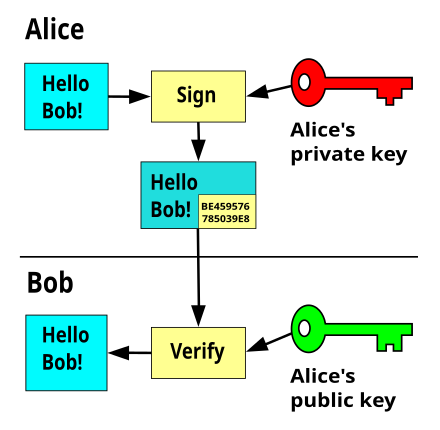
\includegraphics[width=0.3\textwidth]{img/Private_key_signing.svg.png}
    \caption{Digital Signature}
\end{figure}

We need to check the validity of the signature. Padding is required, because:
\begin{itemize}
    \item Without proper padding, certain attacks (such as \textbf{existential forgery}) can exploit weaknesses in the signature scheme to create forged signatures.
    \item Padding ensures the message \( m \) is properly formatted, making it more secure and resistant to attacks.
    \item The message \( m \) is padded to match the required input size for the cryptographic signature algorithm.
\end{itemize}

\subsubsection{Steps for Padding}

Steps for padding: \( m \): The message, represented in \( t \) bits.
\( N \): The modulus, represented in \( k \) bits, where \( t < k-32 \).

\begin{enumerate}
    \item Pad \( m \) with \textbf{zeros} on the left to make it a multiple of 8 bits.
    \item Add \( \frac{k-t}{8} \) additional bytes on the left:
    \begin{itemize}
        \item Begin with `00`: A leading zero.
        \item Add `01`: A start delimiter.
        \item Insert a sequence of `FF` bytes.
        \item Include `00`: A delimiter before the actual message.
    \end{itemize}
    \item The final padded message \( m \) is:
    \[
    m \leftarrow 00 \parallel 01 \parallel FF \parallel FF \ldots \parallel FF \parallel 00 \parallel m.
    \]
\end{enumerate}

\subsubsection{Forgery Attacks}
\textbf{Prevent Existential Forgery:}
    \begin{itemize}
        \item Existential forgery occurs when an attacker can create a valid-looking signature without the private key.
        \item Proper padding prevents attackers from trivially guessing valid signatures.
    \end{itemize}

Padding also prevents againts \textbf{selective forgery} attacks, where an adversary aims to forge a signature for a specific message $m$ of their choice. 
Suppose we have a signing oracle, which can compute signatures for any message, using the private key.
The adversary wants to obtain a valid signature $s$ of target message $m$. 
She can generate a random message $m_1 \in Z/NZ*$. 
The attacker calculates:
\[ m_2 = \frac{m}{m_1} \pmod{N} \]

This ensures that $m_1 \cdot m_2 = m \pmod{N}$. She queries the signing oracle with $m_1, m_2$ and obtains the signatures $s_1, s_2$:

\[ s_1 = m_1^d \pmod{N} \]
\[ s_2 = m_2^d \pmod{N} \]

Using the property of modular arithmetic,, the signatures can be combined:

\[ s = s_1 \cdot s_2 \pmod{N} \]
\[ s = (m_1^d \cdot m_2^d) \pmod{N} \]
\[ = (m_1 \cdot m_2)^d \pmod{N} \]
\[ = m^d \pmod{N} \]

This gives the valid signature $s$ for the target message $m$.
The attack relies on the multiplicative structure of RSA. By introducing proper padding, the relation 
\[
m = m_1 \cdot m_2 \mod N
\]
is broken, making it impossible to combine \( m_1 \) and \( m_2 \) into \( m \) whi

\subsubsection{Signing Documents}
Challenges of signing large documents include the need to divide the message $m$ 
into smaller blocks if it is too large, adding serial numbers and redundant information to ensure integrity and uniqueness for each block, and the fact that signing and verifying each block individually can be computationally expensive.

Solution: use a hash function. Instead of signing the entire message \(m\), the process is simplified by:
    \begin{itemize}
        \item Computing the hash of the message \(h(m)\), a fixed-size digest.
        \item Signing the hash \(h(m)\) instead of the full message.
        \item Separate message recovery and Verification
    \end{itemize}

\textbf{Sender's Side (A):}
\begin{enumerate}
    \item \textbf{Message Preparation:} The sender \(A\) computes the hash of the message: \(h(M)\).
    \item \textbf{Generate the Signature:} The sender uses their private key \(D_{SA}\) to sign the hash \(h(M)\), creating the digital signature \(S_{SA}(M)\).
    \item \textbf{Transmit the Signed Message:} The sender sends \(M\) (the original message) and \(S_{SA}(M)\) (the signature) to the receiver.
\end{enumerate}

\textbf{Receiver's Side (B):}
\begin{enumerate}
    \item \textbf{Hash Verification:} The receiver computes the hash of the received message \(M'\): \(h(M')\).
    \item \textbf{Verify the Signature:}
    \begin{itemize}
        \item The receiver uses the sender's public key \(P_A\) to decrypt the signature \(S_{SA}(M)\), obtaining \(h(M)\).
        \item Compare \(h(M')\) (newly computed) with \(h(M)\) (extracted from the signature).
        \item If they match, the message \(M'\) is verified as authentic.
    \end{itemize}
    \item \textbf{Result:}
    \begin{itemize}
        \item If \(h(M') = h(M)\), verification succeeds.
        \item Otherwise, verification fails.
    \end{itemize}
\end{enumerate}


\begin{figure}[h!]
    \centering
    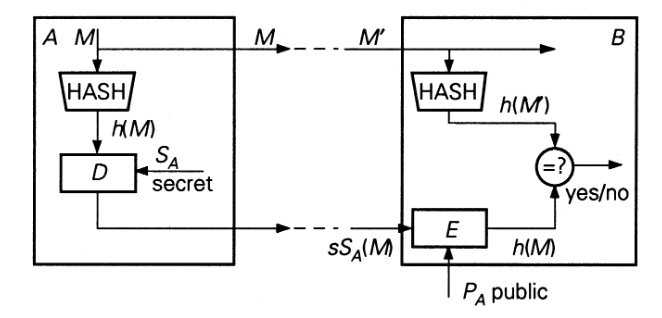
\includegraphics[width=0.5\textwidth]{img/signing.png}
    \caption{\textbf{Sender Side:}
\(M\) is hashed (\(h(M)\)), and the private key generates the signature \(S_{SA}(M)\).
Both \(M\) and \(S_{SA}(M)\) are sent to the receiver.
\textbf{Receiver Side:}
The receiver computes \(h(M')\) and verifies the signature using \(P_A\).
If \(h(M') = h(M)\), the message \(M'\) is validated.}
\end{figure}

\subsubsection{Requirements for the Hash Function}
\begin{itemize}
    \item \textbf{Preimage resistance:} Adversary should not be able to cook her own signature for a message of her choice
    \item \textbf{Second preimage resistance:} Attacker can find another message for a valid signature
    \item \textbf{Collision resistance:} The signer generates two messages with $H(m) = H(m')$ and releases $(m,s)$. Later, she claims $(m',s)$ (repudiation)
\end{itemize}
\Comment{more explanation here}

\subsection{More on the security of RSA}
\begin{itemize}
    \item Knowledge of $d$ and factoring: if you know $d$, you can factor $N$ using the Las Vegas algorithm
    \item Knowledge of $\phi(N)$ and factoring: if you know $\phi(N)$, you can factor $N$
    \item Shared modulus $N$ is \emph{not} a good idea!
    \item Use a small public exponent $e$: using CRT, RSA can be broken. Thus padding is important
    \item More attacks exist (see slides)
\end{itemize}

\subsubsection{Knowledge of \texorpdfstring{$\phi(N)$}{phi(N)} and factoring}
\[ \phi(N) = (p-1)(q-1) = N - (p+1) + 1\]
\[ S = N + 1 - \phi \]
\[ S = p + q \]

\[f(X) = (X - p)\cdot (X - q) = X^2 - S \cdot X + N\]
Then:

\[ p = \frac{S + \sqrt{S^2 - 4\cdot N}}{2} \]
\[ q = \frac{S - \sqrt{S^2 - 4\cdot N}}{2} \]

\subsubsection{Use of a Shared Modulus}
There are two people sharing the same modulus. Two cases:
\begin{enumerate}
    \item Attacker shares the modulus with another person. From $d_1$, the attacker can compute $p$ and $q$. Then the attacker computes $d_2$ from $e_2$ (public key), $p$ and $q$.
    \item Attacker is not one of the two people
    \[ c_1 = m^{e_1} \pmod{N} , \quad t_1 \leftarrow e_1^{-1} \pmod{e_2}\]
    \[ c_2 = m^{e_2} \pmod{N} , \quad t_2 \leftarrow (t_1 \cdot e_1^{-1} -1) / e_2\]
    
    Then:
    \[ c_1^{t_1} \cdot c_2^{t_2} = m^{e_1 \cdot t_1}mm^{-e_2 \cdot t_2} \]
    \[ = m^{1 + e_2 \cdot t_2}mm^{-e_2 \cdot t_2} \]
    \[ = m^{e_1 \cdot t_1 -e_2 \cdot t_2} \]
    \[ = m^1 = m\]
\end{enumerate}

\subsubsection{Use of a Small Public Exponent}
For fast computation, choosing a small public exponent is common.
However, this can lead to attack, particularly when the same message $m$ 
is encrypted under different public keys $N_1, N_2, N_3$.
This is because the ciphertexts $(c_1, c_2, c_3)$ do not involve any randomness in the encryption process (as is the case in textbook RSA). \\

For example, if $e = 3$, then:

\[ c_1 = m^3 \pmod{N_1} \]
\[ c_2 = m^3 \pmod{N_2} \]
\[ c_3 = m^3 \pmod{N_3} \]

Since the moduli are distinct (and therefore coprime), the CRT can be used to comhine the ciphertexts 
and reconstruct the original message $m^3$ modulo $N_1 \cdot N_2 \cdot N_3$. 
Because $m^3 < N_1 \cdot N_2 \cdot N_3$, the modular reduction has no effect (no modulus wrapping).
So then, $X= m^3$ and $X^{1/3} = m$.
Thus, taking the cube root of this value yields the original message $m$.

\[ X = c_i \pmod{N_i} \  \text{for} \ i = 1,2,3 \]
\[ X = m^3 \pmod{N_1 \cdot N_2 \cdot N_3} \]

An attacker can now decrypt the message $m$ without knowing the private keys. \\

Another example taken from assignment 3: \\

A grade between 10 and 100 is encrypted as ciphertext $c = 300763$, with public key $(N,e ) = \\
(0x009026120d59a38f00 \cdots bc859f590645eb0f77196b, 3)$, where the modulo is encoded as a hexidecimal number. \\

Note that the encryptoion exponent $e = 3$ is very small, $e << N$. If $m^e < N$, then the ciphertext 
$c = m^e \pmod{N}$ is the same as $m^e$. This is because the modulus $N$ is so large that the cube of any number less than $N$ is less than $N^2$ (the value doesn't wrap around N). \\

We can easily compute the plain text using the cube root of the ciphertext:

\[ c = m^3 \]
\[ m = \sqrt[3]{c} = \sqrt[3]{300763} = 67\]

This value lies within the range [10, 100], so the plaintext is 67. So, this scheme is \emph{very insecure}.

\subsubsection{Why can't we compute the private key from the public key?}
Say we have the public key $(e,N)$, why can I not just get the private key $d$ by computing $d$ as the modular inverse of $e$ and $\phi(N)$? \\

To find the modular inverse of $e$ modulo $\phi(N)$, we need the prime factorization of $N$. 
For relatively small $N$, this is easy, or we can code it (e.g., in Haskell using number theory).
But RSA uses 2048-bit $N$, finding these factors is computationally challenging.
The performance of the code will degrade exponentially as $N$ grows. \\

Factoring $N$ into $p$ and $q$ is the central hard problem that RSA depends on. Efficient algorithms for factoring $N$ would break RSA encryption (quantum computers).
Without knowing $p$ and $q$, you cannot calculate $\phi(N)$. 
These are kept private and are \textbf{never included in the public key}. 
During RSA key generation, $p$ and $q$ are randomly chosen large prime numbers and discarded after $d$ is computed (in many implementations), reducing the risk of leakage.


\newpage

\end{document}


